\chapterimage{orange2.jpg}
\chapterspaceabove{6.75cm} 
\chapterspacebelow{7.25cm} 
\chapter{Complex Number}
In \autoref{sec:number}, we introduced the categorization of numbers. This chapter will unveil the
most special subset of number that we have known, which is complex number. Complex number is a powerful
mathematical tool for Computer Science, especially for some machine learning algorithms and computer graphics.

In the 18th century, some mathematicians are confused by the roots of equations, especially  high-ordered equation.
In some cases, they have to get the square root of a negative number, which is non-existent in the real number filed.
In this context, mathematicians extend their knowledge to complex number. For equations such as $x^2 = -1$,
we can easily find out that the root is $\sqrt{-1}$, which is not defined for all real numbers. Mathematicians
define $\sqrt{-1}$ as \textbf{Imaginary Number}, denoted by $i$.
\begin{definition}[imaginary Number]
    The equation $x^2 = -1$ is used to define imaginary number $i$, which gives $i^2 = -1$. The two roots are $i$
    and $-i$ respectively.
\end{definition}

Formally, a compex number is defined as:
\begin{definition}
    A complex number is an expression of the form \(a + bi\), where \(a\) and \(b\) are real numbers.
The set of all complex numbers is denoted by \(\mathbb{C}\). That is,
\[
\mathbb{C} = \{ a + bi : a, b \in \mathbb{R} \}
\]
The letter \(z\) is often used to denote a complex number.
\begin{itemize}
    \item If \( a = 0 \), then \( z = bi \) is said to be an imaginary number.
    \item If \( b = 0 \), then \( z = a \) is a real number.
\end{itemize}
The real numbers and the imaginary numbers are subsets of \( \mathbb{C} \)
\end{definition}

\begin{definition} [Real and Imaginary Part]
    For a complex number \( z = a + bi \), we define
\[
\text{Re}(z) = a \quad \text{and} \quad \text{Im}(z) = b
\]
where \(\text{Re}(z)\) is called the \textit{real part} of \(z\), and \(\text{Im}(z)\) is called the \textit{imaginary part} of \(z\).

\textbf{Note:} Both \(\text{Re}(z)\) and \(\text{Im}(z)\) are real numbers. That is, \(\text{Re}: \mathbb{C} \rightarrow \mathbb{R}\) and \(\text{Im}: \mathbb{C} \rightarrow \mathbb{R}\).
\end{definition}    
Sometimes we need to represent or simplify a given number to complex number. refer to the following examples
\begin{example}
    \textbf{a} Represent \(\sqrt{-5}\) as an imaginary number. \quad
    \textbf{b} Simplify \(2\sqrt{-9} + 4i\).
\end{example}
\textbf{Solution}

\textbf{a} \(\sqrt{-5} = \sqrt{5} \times (-1)\) \\
\phantom{\textbf{a}} \(= \sqrt{5} \times \sqrt{-1}\) \\
\phantom{\textbf{a}} \(= i\sqrt{5}\)

\textbf{b} \(2\sqrt{-9} + 4i = 2\sqrt{9} \times (-1) + 4i\) \\
\phantom{\textbf{b}} \(= 2 \times 3 \times i + 4i\) \\
\phantom{\textbf{b}} \(= 6i + 4i\) \\
\phantom{\textbf{b}} \(= 10i\)
\section{Algebra of Complex Number} 
This section discusses operations of complex number and some of its algebraic properties.
For rationals, we have \begin{itemize}
    \item \textbf{Commutative Law of Addition}
    \[ a + b = b + a \]
    
    \item \textbf{Commutative Law of Multiplication}
    \[ ab = ba \]
    
    \item \textbf{Associative Law of Addition}
    \[ a + (b + c) = (a + b) + c \]
    
    \item \textbf{Associative Law of Multiplication}
    \[ a(bc) = (ab)c \]
    
    \item \textbf{Distributive Law}
    \[ (a + b)c = ac + bc, \]
\end{itemize}

for any rationals \( a \), \( b \), and \( c \).

These basic rules are still available for complex number.

\begin{definition}[Addition and Subtraction of Complex Number]
    The operations of addition and subtraction of complex numbers are given by
\[
(a + bi) \pm (c + di) = (a \pm c) + (b \pm d)i,
\]
\end{definition}

\begin{definition}[Multiplication of Complex Number]
    The multiplication of two complex numbers is defined by
\[
(a + bi)(c + di) = (ac - bd) + (bc + ad)i.
\]
where $i^2=-1$.
\end{definition}

Now let's consider division of complex number. If we write it as a fraction, we have two complex number with real and imaginary parts, which is quite tricky to handle.
In this case we can use the technique to deal with fraction with root denominator, rationalization, to cancel the imaginary part in the denominator, as $i^2=-1$.
\begin{definition}[Division of Complex Number]
    The division of complex numbers is given by
\[
\frac{a + bi}{c + di} := \frac{ac + bd}{c^2 + d^2} + \frac{bc - ad}{c^2 + d^2}i \quad (\text{if } c^2 + d^2 \neq 0).
\]
\end{definition}

\begin{example}
    Find the quotient
\[
\frac{(6 + 2i) - (1 + 3i)}{(-1 + i) - 2}.
\]
\end{example}
\textbf{Solution.}
\begin{align*}
\frac{(6 + 2i) - (1 + 3i)}{(-1 + i) - 2} &= \frac{5 - i}{-3 + i} = \frac{5 - i}{-3 + i} \cdot \frac{(-3 - i)}{(-3 - i)} \\
&= \frac{-15 - 1 - 5i + 3i}{9 + 1} \\
&= \frac{-16 - 2i}{10} \\
&= \frac{-8}{5} - \frac{1}{5}i. 
\end{align*}

\subsection{Exercises}
\begin{exercise}
    Verify the commutative, associative, and distributive laws for complex numbers.
\end{exercise}

\begin{exercise}
    Notice that \(0\) and \(1\) retain their “identity” properties as complex numbers; that is, \(0 + z = z\) and \(1 \cdot z = z\) when \(z\) is complex.
    \begin{enumerate}[label=(\alph*)]
        \item Verify that complex subtraction is the inverse of complex addition (that is, \(z_3 = z_2 - z_1\) if and only if \(z_3 + z_1 = z_2\)).
        \item Verify that complex division, as given in the text, is the inverse of complex multiplication (that is, if \(z_2 \neq 0\), then \(z_3 = z_1 / z_2\) if and only if \(z_3z_2 = z_1\)).
    \end{enumerate}
    \end{exercise}

\begin{exercise}
    Prove that if $z_1z_2=0$, then $z_1=0$ or $z_2=0$.
\end{exercise}

\begin{exercise}
    Show that \(\Re(i z) = -\Im z\) for every complex number \(z\).
\end{exercise}
Hint: Prove using $z=a+bi$ directly.

\begin{exercise}
    Let $\displaystyle k$ be an integer. show that

\begin{equation*}
i^{4k} =1,\ i^{4k+1} =i,\ i^{4k+2} =-1,\ i^{4k+3} =-i
\end{equation*}
and thus evalueate
\begin{equation*}
3i^{11} +6i^{3} +\frac{8}{i^{20}} +i^{-1}
\end{equation*}
\end{exercise}
\begin{proof}
    We know that \( i^2 = -1 \). Therefore, we can express powers of \( i \) in terms of powers of \( -1 \):
\begin{align*}
i^{4k} &= (i^2)^{2k} = (-1)^{2k} = 1, \\
i^{4k+1} &= i^{4k} \cdot i = 1 \cdot i = i, \\
i^{4k+2} &= i^{4k} \cdot i^2 = 1 \cdot (-1) = -1, \\
i^{4k+3} &= i^{4k+2} \cdot i = (-1) \cdot i = -i.
\end{align*}
Now we can evaluate the given expression:

\[
3i^{11} + 6i^3 + \frac{8}{i^{20}} + i^{-1} = 3i^{4(2)+3} + 6i^{4(0)+3} + \frac{8}{i^{4(5)}} + i^{-1}
\]
\[
= 3(-i) + 6(-i) + \frac{8}{1} + \frac{1}{i}
\]
\[
= -3i - 6i + 8 - i \cdot \left( \frac{1}{i} \cdot \frac{i}{i} \right) = -3i - 6i + 8 - \frac{i}{i^2} = -3i - 6i + 8 - \frac{i}{-1} = -3i - 6i + 8 + i
\]
\[
= 8 - 10i
\]
Therefore, the evaluated expression is \( 8 - 10i \).
\end{proof}

\begin{exercise}
    Solve each of the following equations for \( z \).
    \begin{enumerate}[label=(\alph*)]
        \item \( iz = 4 - zi \)
        \item \( \frac{z}{1 - z} = 1 - 5i \)
        \item \( (2 - i)z + 8z^2 = 0 \)
        \item \( z^2 + 16 = 0 \)
    \end{enumerate}
\end{exercise}


\begin{exercise}
    The complex numbers \( z_1, z_2 \) satisfy the system of equations
\begin{align*}
    (1 - i)z_1 + 3z_2 &= 2 - 3i, \\
    iz_1 + (1 + 2i)z_2 &= 1.
\end{align*}
Find \( z_1, z_2 \).
\end{exercise}
Hint: To find \( z_1 \) and \( z_2 \), we solve the system of equations and find that
\[ z_1 = 1 + i \]
\[ z_2 = -i \]

\begin{exercise}
    The straightforward method of computing the product \((a + bi)(c + di) = (ac - bd) + i(bc + ad)\) requires four (real) multiplications (and two signed additions). On most computers multiplication is far more time-consuming than addition. Devise an algorithm for computing \((a + bi)(c + di)\) with only three multiplications (at the cost of extra additions). 
    \begin{itemize}
        \item Write this algorithm in pseudocode
    \end{itemize}
\end{exercise}

\noindent Hint: Start with \((a + b)(c + d)\), this is calleded "Karatsuba's algorithm"

\noindent \textbf{Solution:}
\begin{algorithm}
    \caption{Karatsuba's algorithm for multiplying two complex numbers}
    \begin{algorithmic}[1]
    \Procedure{KaratsubaMultiply}{$a, b, c, d$}
    \State $ac \gets a \cdot c$
    \State $bd \gets b \cdot d$
    \State $abcd \gets (a + b) \cdot (c + d)$
    \State $real \gets ac - bd$
    \State $imag \gets abcd - ac - bd$
    \State \Return $real + imag \cdot i$
    \EndProcedure
    \end{algorithmic}
    \end{algorithm}

\section{Point representation of Complex Number}
This section delves into the representation of Complex Number in the Cartesian coordinate, with which we are 
already quite familiar. In this system, we use ordered pairs like $(a,b)$ to show the position of a given point.
In the study of complex number, we can draw all complex number on a Cartesian coordinate which we call \textbf{Complex Plane}.

\begin{figure}[H]
    \centering
    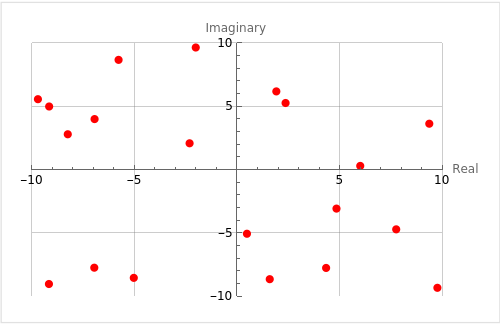
\includegraphics{complexplane.png}
    \caption{Complex Plane}
\end{figure}

\begin{definition}[Complex Plane]
    The complex plane is a two-dimensional space where each point represents a complex number. The horizontal axis represents the real part of the number, and the vertical axis represents the imaginary part. This allows for a geometric interpretation of complex numbers.
\end{definition}
Now that we have point representation on the complex plane, we can gauge the length of a complex number, which we call
\textbf{absolute value} or \textbf{modulus}, as what we do to vectors.
\begin{definition}[Modulus of Complex Number]
    The absolute value or modulus of the number \( z = a + bi \) is denoted by \( |z| \) and is given by
\[ |z| := \sqrt{a^2 + b^2}. \]
\end{definition}
In particular,
\[ |0| = 0, \quad \left|\frac{i}{2}\right| = \frac{1}{2}, \quad |3 - 4i| = \sqrt{9 + 16} = 5. \]
Similarly, we can also gain the distance between two complex numbers in the plane by taking them as two points.
\begin{definition}[Distance between Complex Number]
    Let \( z_1 = a_1 + b_1i \) and \( z_2 = a_2 + b_2i \). 
    \begin{equation}
        |z_1 - z_2| = |(a_1 - a_2) + (b_1 - b_2)i| = \sqrt{(a_1 - a_2)^2 + (b_1 - b_2)^2}
    \end{equation}
\end{definition}
We can use this property to describe curves in the plane.
\begin{example}
    Draw the area that satisfies $|z-z_0|=1$, where $z_0 = 2+2i$.
\end{example}

This set consists of all points $z$ whose distance from $z_0$ is $r$.
\begin{figure}[H]
    \centering
    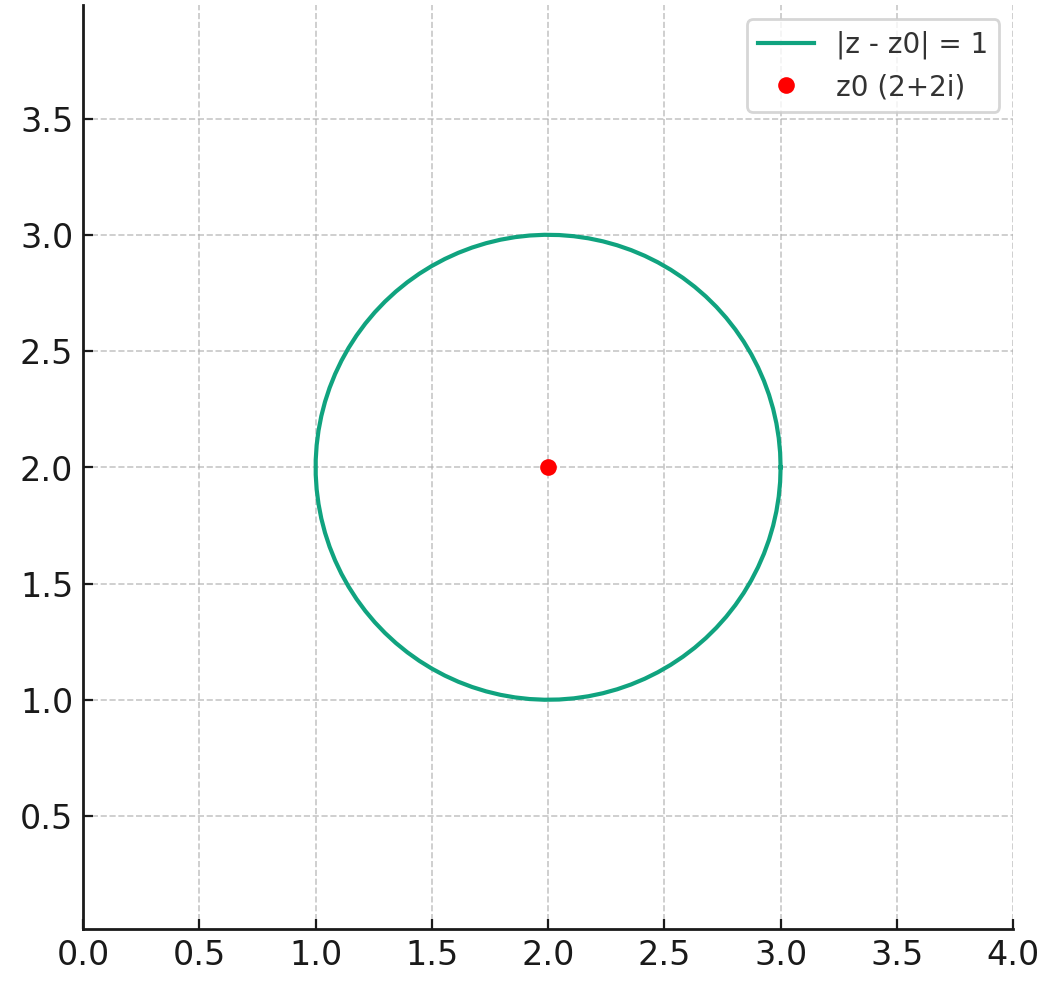
\includegraphics[width = 0.5\textwidth]{locus1.png}
\end{figure}
\begin{example}
    Describe the set of points \( z \) that satisfy the equations

\begin{enumerate}
\item[(a)] \( |z + 2| = |z - 1| \),
\item[(b)] \( |z - 1| = \text{Re} \, z + 1 \).
\end{enumerate}
\end{example}
\textbf{Solution.}

\begin{itemize}
    \item[(a)] A point \( z \) satisfies Eq. (a) if and only if it is equidistant from the points \( -2 \) and \( 1 \). Hence, Eq. (a) is the equation of the perpendicular bisector of the line segment joining \( -2 \) and \( 1 \); that is, Eq. (a) describes the line \( x = -\frac{1}{2} \).

    A more routine method for solving Eq. (a) is to set \( z = x + iy \) in the equation and perform the algebra:
    \begin{align*}
        |z + 2| &= |z - 1|, \\
        |x + iy + 2| &= |x + iy - 1|, \\
        (x + 2)^2 + y^2 &= (x - 1)^2 + y^2, \\
        4x + 4 &= -2x + 1, \\
        x &= -\frac{1}{2}.
    \end{align*}

    \item[(b)] The geometric interpretation of Eq. (b) is less obvious, so we proceed directly with the mechanical approach and derive
    $$\sqrt{(x-1)^2} + y^2 = x+1 \iff y^2 = 4x$$
    which is a parabola.
\end{itemize}
Another important concept is \textbf{complex conjugate}.

Geometrically, the conjugate of a complex number is its reflection on the x-axis.
\begin{wrapfigure}{r}{0.5\textwidth}
    \centering
    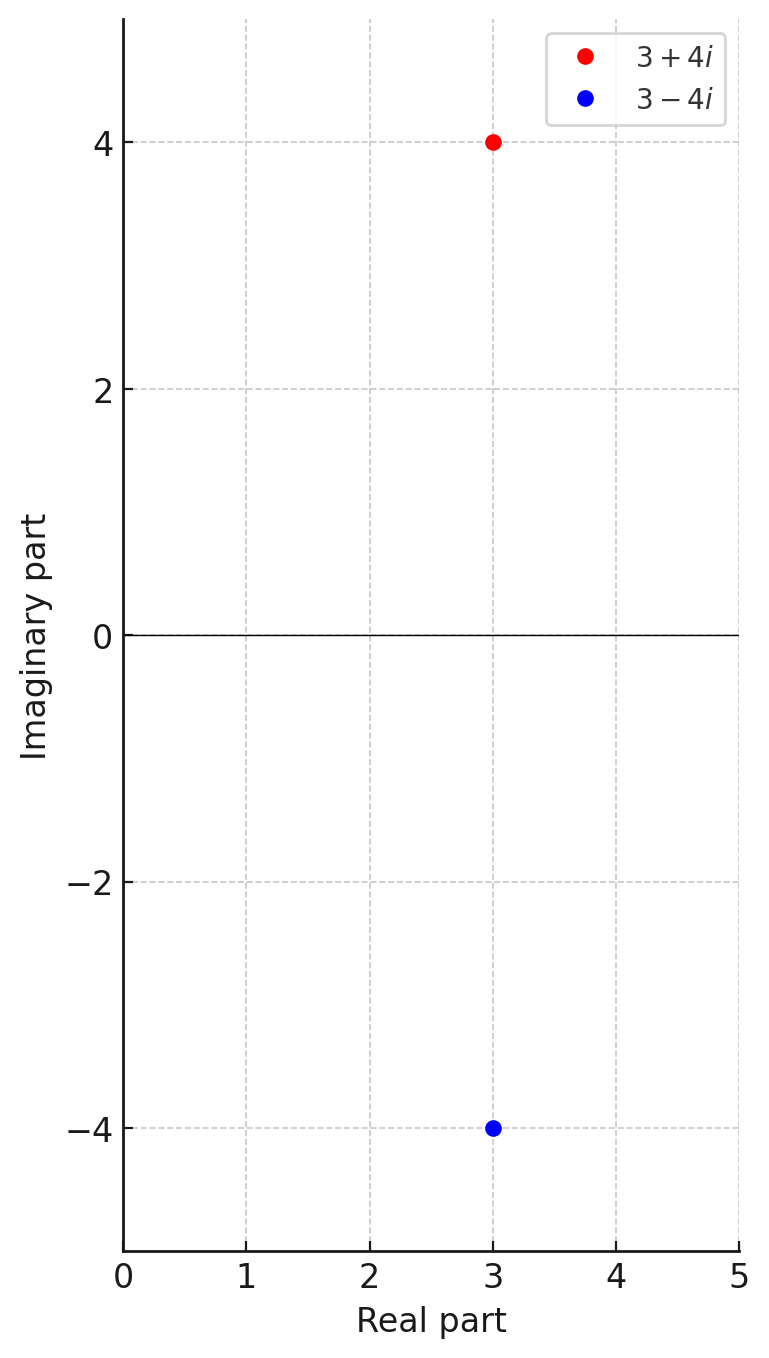
\includegraphics[width=0.48\textwidth]{conjugate.png}
    \caption{Complex Conjugate}
  \end{wrapfigure}
  The complex conjugate of the number $z = a+bi$ is denoted by $\bar{z} = a-bi $.
  It follows that \( z = \bar{z} \) if and only if \( z \) is a real number. Also, it is clear that the conjugate of the sum (difference) of two complex numbers is equal to the sum (difference) of their conjugates; that is,

$$z_1 + z_2 = \bar{z}_1 + \bar{z}_2$$

$$\quad z_1 - z_2 = \bar{z}_1 - \bar{z}_2$$

We also have:
$$\bar{(z_1z_2)} = \bar{z_1} \bar{z_2}$$
and
$$\begin{aligned}\overline{\left(\frac{z_1}{z_2}\right)}&=\frac{\bar{z_1}}{\bar{z_2}}\quad(z_2\neq0);\\\operatorname{Re}z&=\frac{z+\bar{z}}2;\\\operatorname{Im}z&=\frac{z-\bar{z}}{2i};\end{aligned}$$
The proof is not very complex, and is therefore exercises for this section.
\\
\subsection{Exercises}


\begin{exercise}
    Describe the set of points \( z \) in the complex plane that satisfies each of the following.
    \begin{enumerate}
        \item[\textbf{(a)}] \( \text{Im} \, z = -2 \)
        \item[\textbf{(b)}] \( |z - 1 + i| = 3 \)
        \item[\textbf{(c)}] \( |2z - i| = 4 \)
        \item[\textbf{(d)}] \( |z - 1| = |z + i| \)
        \item[\textbf{(e)}] \( |z| = \text{Re} \, z + 2 \)
        \item[\textbf{(f)}] \( |z - 1| + |z + 1| = 7 \)
        \item[\textbf{(g)}] \( |z| = 3|z - 1| \)
        \item[\textbf{(h)}] \( \text{Re} \, z \geq 4 \)
        \item[\textbf{(i)}] \( |z - i| < 2 \)
        \item[\textbf{(j)}] \( |z| > 6 \)
      \end{enumerate}
\end{exercise}
\begin{proof}
    Here we describe the set of points \( z \) in the complex plane that satisfies each of the following conditions:
    
    \begin{enumerate}
      \item[\textbf{(a)}] For \( \text{Im} \, z = -2 \), the Cartesian equation is \( y = -2 \).
      \item[\textbf{(b)}] For \( |z - 1 + i| = 3 \), the Cartesian equation is \( (x - 1)^2 + (y + 1)^2 = 9 \).
      \item[\textbf{(c)}] For \( |2z - i| = 4 \), the Cartesian equation is \( (2x)^2 + (2y - 1)^2 = 16 \).
      \item[\textbf{(d)}] For \( |z - 1| = |z + i| \), the Cartesian equation is \( (x - 1)^2 + y^2 = x^2 + (y + 1)^2 \).
      \item[\textbf{(e)}] For \( |z| = \text{Re} \, z + 2 \), the Cartesian equation is \( x^2 + y^2 = x + 2 \).
      \item[\textbf{(f)}] For \( |z - 1| + |z + 1| = 7 \), this is the equation of an ellipse with foci at (1,0) and (-1,0).
      \item[\textbf{(g)}] For \( |z| = 3|z - 1| \), the Cartesian equation is \( x^2 + y^2 = 3(\sqrt{(x - 1)^2 + y^2}) \).
      \item[\textbf{(h)}] For \( \text{Re} \, z \geq 4 \), the Cartesian equation is \( x \geq 4 \).
      \item[\textbf{(i)}] For \( |z - i| < 2 \), the Cartesian equation is \( (x)^2 + (y - 1)^2 < 4 \).
      \item[\textbf{(j)}] For \( |z| > 6 \), the Cartesian equation is \( x^2 + y^2 > 36 \).
    \end{enumerate}
    \end{proof}

    \begin{exercise}
        Prove that if \( \overline{z}^2 = z^2 \), then \( z \) is either real or pure imaginary.
        \end{exercise}
        
        \begin{proof}
        Let \( z = a + bi \) where \( a \) and \( b \) are real numbers and \( i \) is the imaginary unit. Then \( \overline{z} = a - bi \). 
        
        According to the premise:
        \[ \overline{z}^2 = (a - bi)^2 = a^2 - 2abi + b^2i^2 = a^2 - 2abi - b^2 \]
        \[ z^2 = (a + bi)^2 = a^2 + 2abi + b^2i^2 = a^2 + 2abi - b^2 \]
        
        For \( \overline{z}^2 \) to equal \( z^2 \), the real parts and the imaginary parts of \( \overline{z}^2 \) and \( z^2 \) must be equal, thus:
        \[ a^2 - b^2 = a^2 - b^2 \]
        \[ -2ab = 2ab \]
        
        The real parts are already equal. For the imaginary parts to be equal, \( -2ab \) must equal \( 2ab \), which is only possible if \( ab = 0 \). This means that either \( a = 0 \) or \( b = 0 \) (or both).
        
        If \( a = 0 \), then \( z \) is pure imaginary. If \( b = 0 \), then \( z \) is real. Hence, if \( \overline{z}^2 = z^2 \), \( z \) must be either real or pure imaginary.
        \end{proof}

        \begin{exercise}
            Show that:
            \begin{itemize}
                \item$\lvert z_1z_2 \rvert = \lvert z_1 \rvert \lvert z_2 \rvert$ \quad (the modulus of a product is the product of the moduli)
                \item $\left\lvert \frac{z_1}{z_2} \right\rvert = \frac{\lvert z_1 \rvert}{\lvert z_2 \rvert}$ \quad (the modulus of a quotient is the quotient of the moduli)
                \item $\lvert z_1 \rvert + \lvert z_2 \rvert \leq \lvert z_1 + z_2 \rvert$ \quad (triangle inequality)
              \end{itemize}
        \end{exercise}
        
        \begin{exercise}
            Show that:
            \begin{itemize}
                \item $z_1 + z_2 = \overline{z_1} + \overline{z_2}$
                \item $z_1z_2 = \overline{z_1} \, \overline{z_2}$
                \item $\overline{z}z = \lvert z \rvert^2$
                \item $z + \overline{z} = 2Re(z)$
                \item $kz = \overline{kz}$, for $k \in \mathbb{R}$
              \end{itemize}
        \end{exercise}
        \begin{exercise}
            Prove that \( \overline{z}^k = (\overline{z^k}) \) for every integer \( k \) (provided \( z \neq 0 \) when \( k \) is negative).
            \end{exercise}
            
            \begin{proof}
            Consider a complex number \( z = a + bi \), where \( a \) and \( b \) are real numbers and \( i \) is the imaginary unit. The complex conjugate of \( z \) is \( \overline{z} = a - bi \).
            
            The statement is trivially true for \( k = 0 \) and \( k = 1 \). Now let \( k \) be any positive integer.
            
            We proceed by induction on \( k \):
            
            \textbf{Base case} (\( k = 1 \)):
            \[ \overline{z}^1 = \overline{z} = a - bi = \overline{z^1} \]
            The base case holds.
            
            \textbf{Inductive step}:
            Assume the statement is true for \( k \), i.e., \( \overline{z}^k = \overline{z^k} \). We need to show that \( \overline{z}^{k+1} = \overline{z^{k+1}} \).
            \[ \overline{z}^{k+1} = \overline{z}^k \cdot \overline{z} = \overline{z^k} \cdot \overline{z} \]
            Using the property of complex conjugates that \( \overline{zw} = \overline{z} \cdot \overline{w} \), we have:
            \[ \overline{z^k} \cdot \overline{z} = \overline{z^k \cdot z} = \overline{z^{k+1}} \]
            This completes the inductive step.
            
            For negative integers \( k \), we have \( \overline{z}^k = \overline{z^{-k}} = (\overline{z^{-1}})^k = (\overline{z})^k \), since the complex conjugate of a reciprocal is the reciprocal of the complex conjugate, and the induction hypothesis applies.
            
            Therefore, \( \overline{z}^k = (\overline{z^k}) \) for every integer \( k \).
            \end{proof}

            \begin{exercise}\label{conjugate root}
                Let \( a_1, a_2, \ldots, a_n \) be real constants. Show that if \( z_0 \) is a root of the polynomial equation \( z^n + a_1z^{n-1} + a_2z^{n-2} + \ldots + a_n = 0 \), then so is \( \overline{z_0} \).
                \end{exercise}
                
                \begin{proof}
                Suppose \( z_0 \) is a root of the polynomial \( P(z) = z^n + a_1z^{n-1} + a_2z^{n-2} + \ldots + a_n \). This means that:
                \[ P(z_0) = z_0^n + a_1z_0^{n-1} + a_2z_0^{n-2} + \ldots + a_n = 0 \]
                
                Taking the complex conjugate of the entire equation, we have:
                \[ \overline{P(z_0)} = \overline{z_0^n + a_1z_0^{n-1} + a_2z_0^{n-2} + \ldots + a_n} = \overline{0} \]
                
                Since the \( a_i \) are real, \( \overline{a_i} = a_i \), and using the property that \( \overline{z + w} = \overline{z} + \overline{w} \) and \( \overline{zw} = \overline{z}\cdot \overline{w} \), we get:
                \[ \overline{P(z_0)} = \overline{z_0}^n + a_1\overline{z_0}^{n-1} + a_2\overline{z_0}^{n-2} + \ldots + a_n \]
                
                Since \( \overline{0} = 0 \), the equation simplifies to:
                \[ P(\overline{z_0}) = \overline{z_0}^n + a_1\overline{z_0}^{n-1} + a_2\overline{z_0}^{n-2} + \ldots + a_n = 0 \]
                
                Therefore, \( \overline{z_0} \) is also a root of the polynomial \( P(z) \).
                \end{proof}
                \begin{remark}
                    This statement is actually \textbf{Conjugate Root Theorem}, which we will discuss further details about in finding
                    complex roots of equations.
                \end{remark}
            \begin{exercise}
                We have noted that the conjugate \( \overline{z} \) is the reflection of the point \( z \) in the real axis (the horizontal line \( y = 0 \)). Show that the reflection of \( z \) in the line \( ax + by = c \) (where \( a, b, c \) are real) is given by
\[ \frac{2ic    + (b - ai)\overline{z}}{b + ai} \]
            \end{exercise}
            Hint: In general, the reflection of the point \( (x_1, y_1) \) in the line \( ax + by + c = 0 \) given by this formula:
            \[ 
            x_2 = \frac{x_1(b^2 - a^2) - 2aby_1 - 2ac}{a^2 + b^2}
            \]
            \[ 
            y_2 = \frac{y_1(a^2 - b^2) - 2abx_1 - 2bc}{a^2 + b^2}
            \]
            
            \begin{proof}
                Now the reflection of $z = (x, y)$ in the line $ax + by - c = 0$ is $w = u + iv$, $u, v \in \mathbb{R}$, where:
                \begin{align*}
                u &= \frac{x(b^2 - a^2) - 2aby + 2ac}{a^2 + b^2}, \\
                v &= \frac{y(a^2 - b^2) - 2abx + 2bc}{a^2 + b^2}.
                \end{align*}
                Then:
                \begin{align*}
                w = u + vi &= \frac{x(b^2 - a^2) - 2aby + 2ac}{a^2 + b^2} + \frac{y(a^2 - b^2) - 2abx + 2bc}{a^2 + b^2}i. 
                \end{align*}
                Next, we'll prove now:
                \begin{align*}
                w &= \frac{2ic + (b - ai)\overline{z}}{b + ai}.
                \end{align*}
                We'll factorize and simplify $w$ in $(*)$:
                \begin{align*}
                w &= \frac{x(b^2 - a^2) - 2aby + 2ac}{a^2 + b^2} + \frac{y(a^2 - b^2) - 2abx + 2bc}{a^2 + b^2}i \\
                &= \frac{x(b^2 - a^2) - 2aby + 2ac + y(a^2 - b^2)i - 2abxi + 2bci}{a^2 + b^2}.
                \end{align*}
                Simplify more:
                \begin{align*}
                (b^2 - a^2 - 2abi) &= (b - ai)^2, \\
                (a^2i - b^2i - 2ab) &= (-i)(b^2 - a^2 + 2ab) \\
                &= (-i)(b + ai)^2 \quad \left(\text{since } \frac{1}{i} = -i\right), \\
                &= (-i)(b - ai)(b + ai)^2 \\
                &= i(b - ai) \\
                &= i(b - ai)(b + ai).
                \end{align*}
                Now we'll put all of them in the $(1)$,
                \begin{align*}
                w &= \frac{x(b - ai)^2 - yi(b - ai)^2 + 2ci(b - ai)}{b + ai} \\
                &= \frac{(b - ai)x(b - ai) - yi(b - ai) + 2ci}{b + ai} \\
                &= \frac{2ci + (b - ai)\overline{z}}{b + ai}.
                \end{align*}
                Therefore, the reflection of $z$ in the line $ax + by = c$ is:
                \begin{align*}
                w &= \frac{2ic + (b - ai)\overline{z}}{b + ai}.
                \end{align*}
                \end{proof}
               
\section{Vector and Polar Form}
\subsection{Vector Form of Complex Number}
Now that we can express complex numbers as points scattered in the complex plane, we can take them as direction vectors
in the plane as shown in figure \ref{vec}. 
\begin{figure}[H]
    \centering \label{vec}
    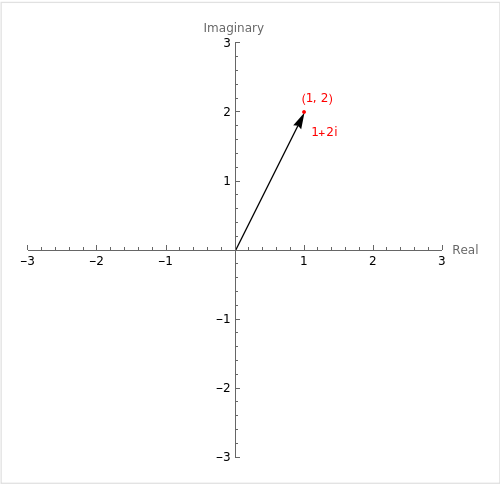
\includegraphics[width = 0.5\textwidth]{complexvector.png}
    \caption{Complex Number as Vector}
\end{figure}
With this, we can apply all possible operations of vectors to complex numbers, such as the \textbf{parallelogram law} as in figure \ref{parrl}.
\begin{figure}[H]
    \centering \label{parrl}
    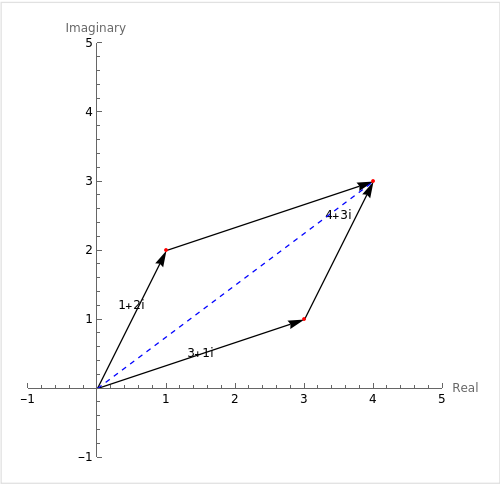
\includegraphics[width = 0.5\textwidth]{paralaw.png}
    \caption{Parallelogram Law}
\end{figure}
Examing this figure, it actually reminds us of a important conclusion mentioned in earlier chapter. If we focus on
the lower triangle of the parallelogram, and denote these two complex numbers as $z_1$ and $z_2$ respectively.
They hold that: $$|z_1+z_2| \leq |z_1|+|z_2|$$
This is exactly the geometrical meaning of triangular inequality as in definition \ref{triangularineq}.
And these are all we need to know about complex number's vector form, as it is not used very common.

\subsection{Polar Form of Complex Number}
This section discusses one of the most commonly used form of complex number. We start with introducing a new coordinate syste.

\subsubsection{The Polar Coordinate}
Polar coordinates provide an alternative to Cartesian coordinates for describing the location of points in a two-dimensional plane. While Cartesian coordinates use a grid of horizontal and vertical lines to specify a point by its horizontal (x) and vertical (y) distances from an origin, polar coordinates specify a point by its distance from a reference point (called the pole, analogous to the origin) and an angle relative to a reference direction.
\begin{figure}[H]
    \centering \label{polar}
    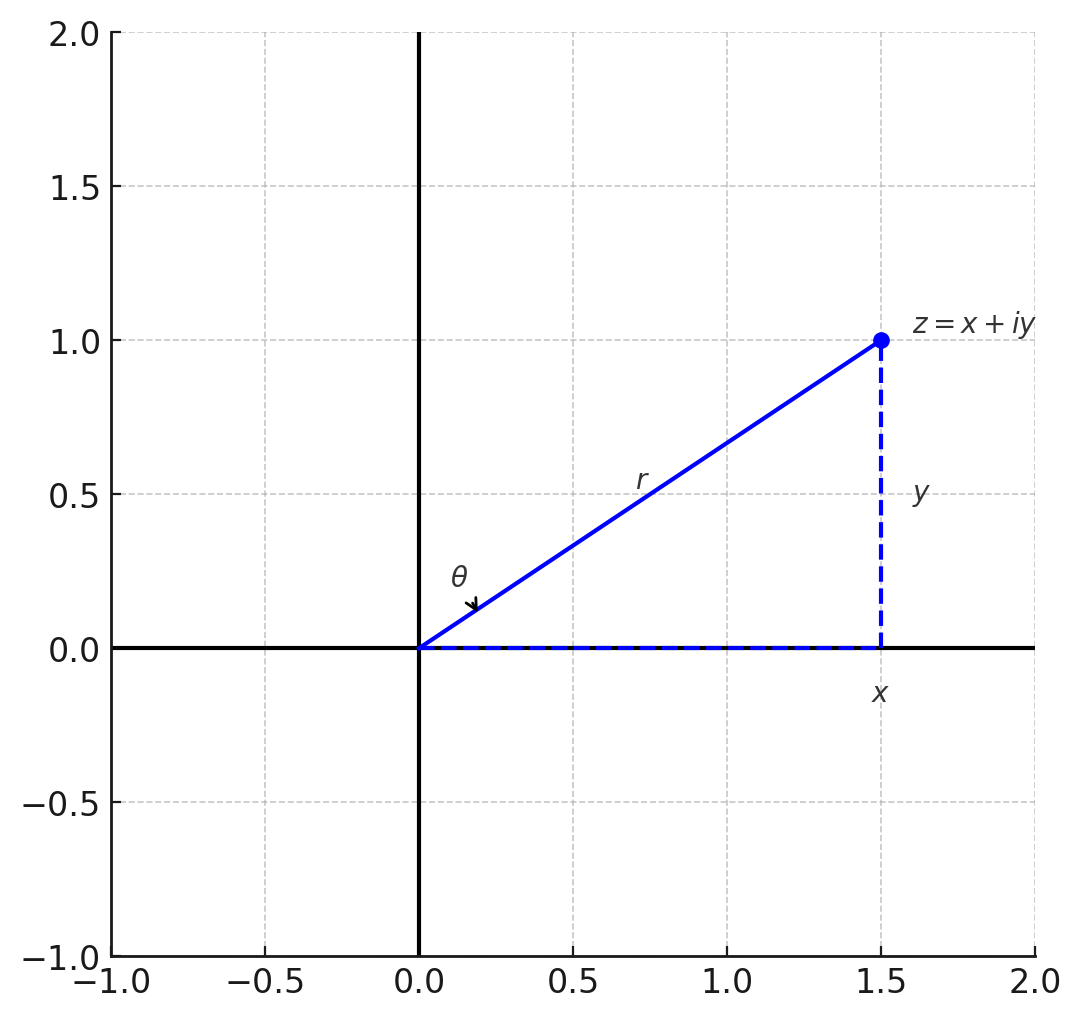
\includegraphics[width = 0.5\textwidth]{polar2.png}
    \caption{Complex Number in Polar Coordinate}
\end{figure}
A point's location in polar coordinates is given as \( (r, \theta) \), where \( r \) is the radial distance from the pole, and \( \theta \) is the angular coordinate, typically measured in radians from the positive x-axis (the reference direction). Polar coordinates are particularly useful in situations where the geometry of a problem has rotational symmetry, making it more natural and simpler to work with angles and radii than with rectangular coordinates.

One of the most common applications of polar coordinates is in the field of trigonometry, complex numbers, and vector calculus, where they provide a more straightforward approach to solving problems involving circular motion, periodic functions, and fields.

\subsubsection{Polar Expression of Complex Number}
Now that we know the existence of polar form, how can we get it from Cartesian form? In the Cartesian coordinate,
the positions are expressed, straightforwardly, in the horizontal and vertical distance to y and x-axis, while in polar
coordinate, we express them using the angle between the line from the origin to the specific position and the horizontal axis, as well
as the length of this line. Is there a mapping or relation between the points in these two types of coordinates? Some clever students
may have noticed that trigonometric functions are the keys here.
we readily derive the equations expressing the rectangular (or Cartesian) coordinates $(x, y)$ in terms of the polar coordinates $(r, \theta)$:
\begin{equation}
x = r \cos \theta, \quad y = r \sin \theta. 
\end{equation}
On the other hand, the expressions for $(r, \theta)$ in terms of $(x, y)$ contain some minor but troublesome complications. Indeed the coordinate $r$ is given, unambiguously, by
\begin{equation}
r = \sqrt{x^2 + y^2} = |z|. 
\end{equation}

However, observe that although it is certainly true that $\tan \theta = \frac{y}{x}$, the natural conclusion
\begin{equation}
\theta = \tan^{-1}\left(\frac{y}{x}\right)
\end{equation}
is \textit{invalid} for points $z$ in the second and third quadrants (since the standard interpretation of the arctangent function places its range in the first and fourth quadrants). Since an angle is fixed by its sine \textit{and} cosine, $\theta$ is uniquely determined by the pair of equations
\begin{equation}
\cos \theta = \frac{x}{|z|}, \quad \sin \theta = \frac{y}{|z|}, 
\end{equation}
And all these lead us to the polar form of a given complex number:
\begin{equation}
    z=x+iy=r(\cos\theta+i\sin\theta)=r\operatorname{cis}\theta
\end{equation}

Considering the circularity of radiant, we introduce the \textbf{argument} of complex number.
\begin{definition}[Arguement of Complex Number] \label{polarform}
In the study of complex numbers, the \emph{argument} of a complex number \( z \), denoted as \( \text{arg}(z) \), is a fundamental concept representing the angle between the positive real axis and the line segment that joins the origin with the point \( z \) in the complex plane. Specifically, if \( z = x + iy \), where \( x \) and \( y \) are real numbers, then \( \text{arg}(z) \) is defined as the angle \( \theta \) in polar coordinates that satisfies \( x = r\cos(\theta) \) and \( y = r\sin(\theta) \), where \( r \) is the magnitude of \( z \). The value of \( \text{arg}(z) \) is usually given in radians and, by convention, is restricted to the interval \( (-\pi, \pi] \), known as the principal value. The argument provides a complete description of the direction in which the point \( z \) lies from the origin, serving as a crucial tool in the fields of complex analysis, phasor calculus in electrical engineering, and in the representation of waves and oscillations.
\end{definition}

\begin{example}
    Find $\arg(1 + \sqrt{3}i)$ and write $1 + \sqrt{3}i$ in polar form.
\end{example}
\textbf{Solutions:}

Note that $r = |1 + \sqrt{3}i| = 2$ and that the equations $\cos\theta = \frac{1}{2}$, $\sin\theta = \frac{\sqrt{3}}{2}$ are satisfied by $\theta = \frac{\pi}{3}$. Hence $\arg(1 + \sqrt{3}i) = \frac{\pi}{3} + 2k\pi, k = 0, \pm1, \pm2, \ldots$ [in particular, $\text{Arg}(1 + \sqrt{3}i) = \frac{\pi}{3}$]. The polar form of $1 + \sqrt{3}i$ is
\[2(\cos\frac{\pi}{3} + i\sin\frac{\pi}{3}) = 2\operatorname{cis}\frac{\pi}{3}.\]

More properties of polar form complex number could be derived with properties of trigonometric identities.
Now suppose we have 
$$z_1=r_1\left(\cos\theta_1+i\sin\theta_1\right),\quad z_2=r_2\left(\cos\theta_2+i\sin\theta_2\right)$$
then we have
$$z_1z_2=r_1r_2\left[(\cos\theta_1\cos\theta_2-\sin\theta_1\sin\theta_2)+i(\sin\theta_1\cos\theta_2+\cos\theta_1\sin\theta_2)\right]$$
which follows that
\begin{equation} \label{polarprod}
    z_1z_2=r_1r_2\left[\cos\left(\theta_1+\theta_2\right)+i\sin\left(\theta_1+\theta_2\right)\right]
\end{equation}

\begin{remark}
The compound angle formula is applied in the proof, which should already been covered in high school
syllabus. You may refer to \href{https://en.wikipedia.org/wiki/List_of_trigonometric_identities}{this link} for further information.
A concise proof is provided below.
\begin{proof}[Proof of the Composite Angle Formulas]
    To prove the sine of the sum of two angles \( \alpha \) and \( \beta \), we can use the unit circle and the definition of sine and cosine.
    
    Consider a unit circle where point \( A \) corresponds to angle \( \alpha \), and point \( B \) corresponds to angle \( \alpha + \beta \). Point \( A \) has coordinates \( (\cos(\alpha), \sin(\alpha)) \), and point \( B \) has coordinates \( (\cos(\alpha + \beta), \sin(\alpha + \beta)) \).
    
    By rotating point \( A \) by angle \( \beta \), we can form a right triangle where the new point, \( C \), has coordinates \( (\cos(\alpha)\cos(\beta) - \sin(\alpha)\sin(\beta), \sin(\alpha)\cos(\beta) + \cos(\alpha)\sin(\beta)) \).
    
    The coordinates of point \( C \) represent the cosine and sine of the sum of angles \( \alpha \) and \( \beta \) due to the rotation. Therefore, we have:
    
    \[
    \sin(\alpha + \beta) = \sin(\alpha)\cos(\beta) + \cos(\alpha)\sin(\beta)
    \]
    \[
    \cos(\alpha + \beta) = \cos(\alpha)\cos(\beta) - \sin(\alpha)\sin(\beta)
    \]
    
    Similarly, by considering the rotation in the opposite direction (subtracting angle \( \beta \) from \( \alpha \)), we can derive the formulas for the sine and cosine of the difference of two angles:
    
    \[
    \sin(\alpha - \beta) = \sin(\alpha)\cos(\beta) - \cos(\alpha)\sin(\beta)
    \]
    \[
    \cos(\alpha - \beta) = \cos(\alpha)\cos(\beta) + \sin(\alpha)\sin(\beta)
    \]
    
    Thus, we have proven the composite angle formulas for sine and cosine.

    \end{proof}
\end{remark}

The abbreviated version of Eq. \ref{polarprod} reads as follows:
\[
\overline{z_1z_2} = (r_1 \operatorname{cis} \theta_1)(r_2 \operatorname{cis} \theta_2) = (r_1r_2) \operatorname{cis} (\theta_1 + \theta_2)
\]
and we see that

\textbf{The modulus of the product is the product of the moduli:}
\[
|\overline{z_1z_2}| = |z_1||z_2| \quad (= r_1r_2);
\]


\textbf{The argument of the product is the sum of the arguments:}
\[
\arg \overline{z_1z_2} = \arg z_1 + \arg z_2 \quad (= \theta_1 + \theta_2).
\]
As division is the inverse of multiplication, we can get the following statements by similar method:
\begin{equation} \label{5.8}
    \frac{z_{1}}{z_{2}}=\frac{r_{1}}{r_{2}}\left[\cos\left(\theta_{1}-\theta_{2}\right)+i\sin\left(\theta_{1}-\theta_{2}\right)\right]=\frac{r_{1}}{r_{2}}\mathrm{cis}\left(\theta_{1}-\theta_{2}\right)
\end{equation}
\begin{equation}\label{5.9}
    \arg\left(\frac{z_{1}}{z_{2}}\right)=\arg z_{1}-\arg z_{2} 
\end{equation}
\begin{equation}\label{5.10}
    \left|\frac{z_1}{z_2}\right|=\frac{|z_1|}{|z_2|}
\end{equation}
\begin{example}
    Write the quotient \( \frac{(1 + i)}{(\sqrt{3} - i)} \) in polar form.
\end{example}
\begin{proof}
    The polar forms for \( 1 + i \) and \( \sqrt{3} - i \) are
    \[
    1 + i = |1 + i| \operatorname{cis}(\arg(1 + i)) = \sqrt{2} \operatorname{cis}\left(\frac{\pi}{4}\right),
    \]
    \[
    \sqrt{3} - i = 2 \operatorname{cis}\left(-\frac{\pi}{6}\right).
    \]
    Hence, from Eq. \ref{5.8}, we have
    \[
    \frac{1 + i}{\sqrt{3} - i} = \frac{\sqrt{2}}{2} \operatorname{cis} \left(\frac{\pi}{4} - \left(-\frac{\pi}{6}\right)\right) = \frac{\sqrt{2}}{2} \operatorname{cis}\left(\frac{5\pi}{12}\right).
    \]
    \end{proof}

\subsection{Exercises}
\begin{exercise}
    Find the following:
    \begin{enumerate}
        \item[(a)] \( \left| \frac{1 + 2i}{-2 - i} \right| \)
        \item[(b)] \( \left| (1 + i)(2 - 3i)(4i - 3) \right| \)
        \item[(c)] \( \left| \frac{i(2 + i)^3}{(1 - i)^2} \right| \)
        \item[(d)] \( \left| \frac{(\pi + i)^{100}}{(\pi - i)^{100}} \right| \)
    \end{enumerate}
\end{exercise}
\begin{exercise}
    Draw the following vectors:
    \begin{enumerate}
        \item[(a)] \( 7 \operatorname{cis}\left(\frac{3\pi}{4}\right) \)
        \item[(b)] \( 4 \operatorname{cis}\left(-\frac{\pi}{6}\right) \)
        \item[(c)] \( \operatorname{cis}\left(\frac{3\pi}{4}\right) \)
        \item[(d)] \( 3 \operatorname{cis}\left(\frac{27\pi}{4}\right) \)
    \end{enumerate}
\end{exercise}
\begin{exercise}
    Find the argument of each of the following complex numbers and write each in polar form:
    \begin{enumerate}
        \item[(a)] \( -\frac{1}{2} \)
        \item[(b)] \( -3 + 3i \)
        \item[(c)] \( -\pi i \)
        \item[(d)] \( -2\sqrt{3} - 2i \)
        \item[(e)] \( (1 - i)(-\sqrt{3} + i) \)
        \item[(f)] \( (\sqrt{3} - i)^2 \)
        \item[(g)] \( \frac{-1 + \sqrt{3}i}{2 + 2i} \)
        \item[(h)] \( \frac{-\sqrt{7}(1 + i)}{\sqrt{3} + i} \)
    \end{enumerate}
\end{exercise}
\begin{exercise}
    Show geometrically that the nonzero complex numbers \( z_1 \) and \( z_2 \) satisfy \( z_1 + z_2 = |z_1| + |z_2| \) if and only if they have the same argument.
\end{exercise}
\begin{proof}
    If \( z_1 \) and \( z_2 \) have the same argument, it follows that:

    We see here if $z_1 = r_1(\cos \theta + i \sin \theta)$, $z_2 = r_2(\cos \theta + i \sin \theta)$, then
\begin{align*}
|z_1 + z_2| &= |r_1(\cos \theta + i \sin \theta) + r_2(\cos \theta + i \sin \theta)| \\
&= |(r_1 + r_2)(\cos \theta + i \sin \theta)| \\
&= r_1 + r_2 = |z_1| + |z_2|
\end{align*}
\end{proof}
\begin{exercise}
    Given the vector \( z \), interpret geometrically the vector \( (\cos \phi + i \sin \phi)z \).
\end{exercise}
\textbf{Solution:}

Let \( z \in \mathbb{C} \), \( z = r(\cos \theta + i \sin \theta) \)

\[
(\cos \phi + i \sin \phi)z = (\cos \phi + i \sin \phi)r(\cos \theta + i \sin \theta)
\]
\[
= r[\cos(\theta + \phi) + i \sin(\theta + \phi)]
\]
\[
= r\operatorname{cis}(\theta + \phi)
\]

Geometrically this: \( r\operatorname{cis}(\theta + \phi) \) means a vector that its length \( r \) and argument is \( \theta + \phi \), we can get it by rotating vector \( z \) about origin through an angle \( \phi \) in the counterclockwise direction.

\begin{exercise}
    Show that $|z_1z_2z_3|=|z_1||z_2||z_3|$ and thus prove 
    $$|\prod_{i=1}^{n} z_i| = \prod_{i=1}^{n} |z_i|$$
    \begin{remark}
        $\prod$ is called pi (upper case) notation. Take it as the sigma notation for multiplication.
    \end{remark}
\end{exercise}
    \begin{proof}
        Consider the complex numbers \( z_1 = r_1(\cos \theta_1 + i\sin \theta_1) \), \( z_2 = r_2(\cos \theta_2 + i\sin \theta_2) \), and \( z_3 = r_3(\cos \theta_3 + i\sin \theta_3) \), where \( r_1, r_2, \) and \( r_3 \) are the moduli of \( z_1, z_2, \) and \( z_3 \) respectively, and \( \theta_1, \theta_2, \) and \( \theta_3 \) are the arguments. The product \( z_1z_2z_3 \) is then given by:
        \[
        z_1z_2z_3 = r_1r_2r_3(\cos(\theta_1 + \theta_2 + \theta_3) + i\sin(\theta_1 + \theta_2 + \theta_3))
        \]
        
        The modulus of this product is:
        \[
        |z_1z_2z_3| = |r_1r_2r_3(\cos(\theta_1 + \theta_2 + \theta_3) + i\sin(\theta_1 + \theta_2 + \theta_3))| = r_1r_2r_3
        \]
        
        Since the moduli of \( z_1, z_2, \) and \( z_3 \) are \( r_1, r_2, \) and \( r_3 \) respectively, it follows that:
        \[
        |z_1z_2z_3| = |z_1||z_2||z_3|
        \]
        
        Now, extend this property to a product of \( n \) complex numbers:
        \[
        \prod_{i=1}^{n} z_i = \prod_{i=1}^{n} r_i(\cos \theta_i + i\sin \theta_i)
        \]
        
        Taking the modulus of both sides:
        \[
        \left|\prod_{i=1}^{n} z_i\right| = \left|\prod_{i=1}^{n} r_i(\cos \theta_i + i\sin \theta_i)\right| = \prod_{i=1}^{n} r_i
        \]
        
        Thus:
        \[
        \prod_{i=1}^{n} |\overline{z_i}| = \prod_{i=1}^{n} |z_i|
        \]
        
        as required.

        MI is also a option:

        \textbf{Base case} (\(n = 1\)): For a single complex number \(z_1\), the statement is trivially true since \(|\overline{z_1}| = |z_1|\).

        \textbf{Inductive step}: Assume the statement holds for \(n = k\), i.e.,
        \[
        \prod_{i=1}^{k} |\overline{z_i}| = \prod_{i=1}^{k} |z_i|
        \]
        Now consider \(n = k + 1\) complex numbers. By the induction hypothesis and the property that the modulus of a product is equal to the product of the moduli for any two complex numbers \(a\) and \(b\), namely \(|ab| = |a||b|\), we have:
        \[
        \prod_{i=1}^{k+1} |\overline{z_i}| = |\overline{z_{k+1}}| \prod_{i=1}^{k} |\overline{z_i}| = |z_{k+1}| \prod_{i=1}^{k} |z_i| = \prod_{i=1}^{k+1} |z_i|
        \]
        Thus, by mathematical induction, the statement is proved for all \(n \in \mathbb{N}\).
        \end{proof}

    \begin{exercise}
        Show that\begin{enumerate}
            \item[(a)] $\text{arg } z_1z_2z_3 = \text{arg } z_1 + \text{arg } z_2 + \text{arg } z_3$
            \item[(b)] $\text{arg } z_1 \overline{z_2} = \text{arg } z_1 - \text{arg } z_2$.
        \end{enumerate}
    \end{exercise}              
    \textbf{Solution:}
    Let $z_1, z_2, z_3 \in \mathbb{C}$,

(a) we'll prove $\text{arg }(z_1z_2z_3) = \text{arg } z_1 + \text{arg } z_2 + \text{arg } z_3$

Let $z_1 = r_1(\cos \theta_1 + i \sin \theta_1)$, where $\text{arg } z_1 = \theta_1$

$z_2 = r_2(\cos \theta_2 + i \sin \theta_2)$, where $\text{arg } z_2 = \theta_2$

$z_3 = r_3(\cos \theta_3 + i \sin \theta_3)$, where $\text{arg } z_3 = \theta_3$

We'll prove $\text{arg } z_1z_2z_3 = \text{arg } z_1 + \text{arg } z_2 + \text{arg } z_3$

At first we'll find $z_1z_2z_3$:

\begin{align*}
    z_1z_2z_3 &= (z_1z_2)z_3 = r_1r_2[\cos(\theta_1 + \theta_2) + i \sin(\theta_1 + \theta_2)]z_3 \\
    &= r_1r_2r_3[\cos(\theta_1 + \theta_2) + i \sin(\theta_1 + \theta_2)](\cos \theta_3 + i \sin \theta_3) \\
    &= r_1r_2r_3[\cos(\theta_1 + \theta_2) \cos \theta_3 - \sin(\theta_1 + \theta_2) \sin \theta_3 \\
    &\quad + i(\sin(\theta_1 + \theta_2) \cos \theta_3 + \cos(\theta_1 + \theta_2) \sin \theta_3)] \\
    &= r_1r_2r_3[\cos(\theta_1 + \theta_2 + \theta_3) + i \sin(\theta_1 + \theta_2 + \theta_3)]
\end{align*}

Therefore, $\text{arg } z_1z_2z_3 = \theta_1 + \theta_2 + \theta_3 = \text{arg } z_1 + \text{arg } z_2 + \text{arg } z_3$.

(b) we'll prove $\text{arg } z_1 \overline{z_2} = \text{arg } z_1 - \text{arg } z_2$

Therefore, $z_2 = r_2(\cos \theta_2 + i \sin \theta_2)$ and hence

\[
\overline{z_2} = r_2(\cos(-\theta_2) + i \sin(-\theta_2)) = r_2(\cos \theta_2 - i \sin \theta_2)
\]

Now we find the argument of $z_1 \overline{z_2}$:

\begin{align*}
    \text{arg } z_1 \overline{z_2} &= \text{arg }[(r_1(\cos \theta_1 + i \sin \theta_1))(r_2(\cos \theta_2 - i \sin \theta_2))] \\
    &= \text{arg }[r_1r_2((\cos \theta_1 \cos \theta_2 + \sin \theta_1 \sin \theta_2) \\
    &\quad + i(\cos \theta_1 \sin \theta_2 - \cos \theta_2 \sin \theta_1))] \\
    &= \text{arg }[r_1r_2(\cos(\theta_1 - \theta_2) + i \sin(\theta_1 - \theta_2))] \\
    &= \theta_1 - \theta_2 \\
    &= \text{arg } z_1 - \text{arg } z_2
\end{align*}

Thus, $\text{arg } z_1 \overline{z_2} = \text{arg } z_1 - \text{arg } z_2$.

\begin{exercise}
    Recall that the dot (scalar) product of two planar vectors $v_1 = (x_1, y_1)$ and $v_2 = (x_2, y_2)$ is given by:
    \[ v_1 \cdot v_2 = x_1x_2 + y_1y_2. \]
\textbf{Show that the dot product of the vectors represented by the complex numbers $z_1$ and $z_2$ is given by}
\[ z_1 \cdot z_2 = Re(\overline{z_1}z_2). \]
\end{exercise}
\begin{proof}
    Let $z_1, z_2 \in \mathbb{C}$.

We can represent $z_1, z_2$ as vectors as follows:
\[ z_1 = (x_1, y_1) = x_1 + y_1j, \quad z_2 = (x_2, y_2) = x_2 + y_2j \]
\[ z_1 \cdot z_2 = (x_1 + y_1j) \cdot (x_2 + y_2j) \]
\[ = x_1x_2 + y_1y_2 + x_1y_2(j \cdot j) + x_2y_1(i \cdot j) \]
\[ = x_1x_2 + y_1y_2 + 0 + 0 \quad (\because i^2 = j^2 = -1, i \cdot j = 0) \]
\[ \therefore z_1 \cdot z_2 = x_1x_2 + y_1y_2 \quad \text{(1)} \]

Now we'll find:
\[ \overline{z_1}z_2 = (x_1 - y_1j)(x_2 + y_2j) = x_1x_2 + y_1y_2 + x_1y_2(-j) - x_2y_1j \]
\[ \therefore Re(\overline{z_1}z_2) = x_1x_2 + y_1y_2 \quad \text{(2)} \]

From (1) and (2) we get:
\[ z_1 \cdot z_2 = Re(\overline{z_1}z_2) = x_1x_2 + y_1y_2 \]
\end{proof}

\begin{exercise}
    We have proven the \textbf{Generalized Triangle Inequality} in last chapter that:
    $$\left|\sum_{k=1}^{n} z_{k}\right| \leq \sum_{k=1}^{n}\left|z_{k}\right|$$
    For complex number$z_1$, $z_2$, and $z_3$, prove that:
    $$\left|\frac{m_{1} z_{1}+m_{2} z_{2}+m_{3} z_{3}}{m_{1}+m_{2}+m_{3}}\right| \leq 1$$
\end{exercise}
\begin{proof}
    
We'll take at first:
\[
\left| \frac{m_1z_1 + m_2z_2 + m_3z_3}{m_1 + m_2 + m_3} \right| = \frac{\left| m_1z_1 + m_2z_2 + m_3z_3 \right|}{\left| m_1 + m_2 + m_3 \right|}
\]

Now we'll find:
\[
\left| m_1z_1 + m_2z_2 + m_3z_3 \right| \leq \left| m_1z_1 \right| + \left| m_2z_2 \right| + \left| m_3z_3 \right| \quad \text{(Triangle inequality)}
\]
\[
= m_1 \left| z_1 \right| + m_2 \left| z_2 \right| + m_3 \left| z_3 \right|
\]
\[
\leq m_1 + m_2 + m_3 \quad (\text{since } m_1, m_2, m_3 > 0 \text{ and } \left| z_1 \right|, \left| z_2 \right|, \left| z_3 \right| \leq 1)
\]
\[
= \left| m_1 + m_2 + m_3 \right|
\]

Therefore:
\[
\left| m_1z_1 + m_2z_2 + m_3z_3 \right| \leq \left| m_1 + m_2 + m_3 \right|
\]
\[
\therefore \left| \frac{m_1z_1 + m_2z_2 + m_3z_3}{m_1 + m_2 + m_3} \right| = \frac{\left| m_1z_1 + m_2z_2 + m_3z_3 \right|}{\left| m_1 + m_2 + m_3 \right|} \leq 1
\]
\end{proof}

\section{Exponential Form}
The other form for complex number is its exponential form with base $e$. Euler's formula relate the exponential
expression to the polar expression. However, the proof of Euler's formula require further knowledge of calculus, such as
Taylor series. You may access \href{https://www.youtube.com/watch?v=mvmuCPvRoWQ&t=78s}{this link} for a proof without
calculus. You can also just skip the proof for now, since it does not affect the problem-solving in this chapter.

\begin{definition}[Euler's Formula]
    \begin{equation}
        e^{i y}=\cos y+i \sin y 
    \end{equation}
\end{definition}
You can relate this formula to the polar form very easily, since the right-hand side is equivalent to$cisy$,
which means $y$ is exactly the principal argument of the complex number, $\theta$.

Euler's Formula enables us to write the polar form of a complex number as
\[
z = r \text{cis} \theta = r(\cos \theta + i \sin \theta) = r e^{i\theta}.
\]
Thus, we can (and do) drop the awkward ``cis'' artifice and use, as the standard polar representation,
\[
z = r e^{i\theta} = \lvert z \rvert e^{\text{arg} z}.
\]
In particular, notice the following identities:
\[
e^{i0} = e^{2\pi i} = e^{-2\pi i} = e^{4\pi i} = e^{-4\pi i} = \cdots = 1,
\]
\[
e^{(\pi/2)i} = i, \quad e^{(-\pi/2)i} = -i, \quad e^{\pi i} = -1.
\]

Observe also that  $\left|e^{i \arg z}\right|=1$  and that Euler's equation leads to the following representations of the customary trigonometric functions:
$$\begin{array}{l}
    \cos \theta=\operatorname{Re} e^{i \theta}=\frac{e^{i \theta}+e^{-i \theta}}{2}, \\
    \sin \theta=\operatorname{Im} e^{i \theta}=\frac{e^{i \theta}-e^{-i \theta}}{2 i} .
    \end{array}$$

\begin{proof}
    We start with Euler's formula which states that for any real number \( \theta \),
\begin{equation}
    e^{i\theta} = \cos(\theta) + i\sin(\theta).
\end{equation}
The complex conjugate of \( e^{i\theta} \) is \( e^{-i\theta} \), which gives us
\begin{equation}
    e^{-i\theta} = \cos(-\theta) + i\sin(-\theta) = \cos(\theta) - i\sin(\theta),
\end{equation}
since cosine is an even function, \( \cos(-\theta) = \cos(\theta) \), and sine is an odd function, \( \sin(-\theta) = -\sin(\theta) \).

To derive the expression for the cosine function, we take the sum of \( e^{i\theta} \) and \( e^{-i\theta} \), and divide by 2:
\begin{equation}
    \cos(\theta) = \frac{e^{i\theta} + e^{-i\theta}}{2}.
\end{equation}
This is because the imaginary parts \( i\sin(\theta) \) and \( -i\sin(\theta) \) cancel each other out, leaving the sum of \( \cos(\theta) + \cos(\theta) \), which is then divided by 2.

To derive the expression for the sine function, we take the difference of \( e^{i\theta} \) and \( e^{-i\theta} \), and divide by \( 2i \):
\begin{equation}
    \sin(\theta) = \frac{e^{i\theta} - e^{-i\theta}}{2i}.
\end{equation}
Here, the real parts \( \cos(\theta) - \cos(\theta) \) cancel out, leaving the difference of \( i\sin(\theta) - (-i\sin(\theta)) \) which is \( 2i\sin(\theta) \), and then dividing by \( 2i \) yields \( \sin(\theta) \).

This completes the derivation of the exponential forms of the sine and cosine functions.
\end{proof}

The rules derived in definition \ref{polarform} for multiplying and dividing complex numbers in polar form now find very natural expressions:
\begin{equation}
    z_1z_2 = (r_1e^{i\theta_1})(r_2e^{i\theta_2}) = (r_1r_2)e^{i(\theta_1+\theta_2)},
\end{equation}
\begin{equation}
    \frac{z_1}{z_2} = \frac{r_1e^{i\theta_1}}{r_2e^{i\theta_2}} = \left(\frac{r_1}{r_2}\right)e^{i(\theta_1-\theta_2)},
\end{equation}
and complex conjugation of \( z = re^{i\theta} \) is accomplished by changing the sign of \( i \) in the exponent:
\begin{equation}
    \bar{z} = re^{-i\theta}.
\end{equation}

\begin{example}
    Compute (a) \( \frac{1 + i}{\sqrt{3} - i} \) and (b) \( (1 + i)^{24} \).
\end{example}
\textbf{Solution:}


(a) This quotient was evaluated using the cis operator in Example 1.11 of Sec. 1.3; using the exponential the calculations take the form
\[
1 + i = \sqrt{2} \text{cis} \left(\frac{\pi}{4}\right) = \sqrt{2}e^{i\pi/4},
\]
\[
\sqrt{3} - i = 2 \text{cis} \left(-\frac{\pi}{6}\right) = 2e^{-i\pi/6},
\]
and, therefore,
\[
\frac{1 + i}{\sqrt{3} - i} = \frac{\sqrt{2}e^{i\pi/4}}{2e^{-i\pi/6}} = \frac{\sqrt{2}}{2} e^{i5\pi/12}.
\]

(b) The exponential forms become
\[
(1 + i)^{24} = \left(\sqrt{2}e^{i\pi/4}\right)^{24} = \left(\sqrt{2}^{24}\right)e^{i24\pi/4} = 2^{12} e^{i6\pi} = 2^{12}.
\]
\subsection{De Moivre's Theorem}
De Moivre's Theorem is a fundamental result in complex analysis that connects complex numbers and trigonometry. Named after the French mathematician Abraham de Moivre, the theorem provides a formula for raising complex numbers to any power using polar coordinates.

Given a complex number expressed in polar form as \( z = r(\cos \theta + i\sin \theta) \), where \( r \) is the modulus and \( \theta \) is the argument of the complex number, De Moivre's Theorem states that:
\begin{theorem}[De Moivre's Theorem]
    \begin{equation}
        z^n = r^n (\cos n\theta + i\sin n\theta)
    \end{equation}
    or in exponential form:
    \begin{equation}
        \left(e^{i \theta}\right)^{n}=\underbrace{e^{i \theta} e^{i \theta} \cdots e^{i \theta}}_{(n \text { times })}=e^{i \theta+i \theta+\cdots+i \theta}=e^{i n \theta}
    \end{equation}
\end{theorem}


for any integer \( n \). This elegant relationship not only simplifies the computation of powers of complex numbers but also lays the foundation for finding roots of complex numbers.

The theorem is particularly useful because it transforms a potentially difficult multiplication problem into a much simpler form by taking advantage of the properties of exponential functions and Euler's formula, which expresses complex exponentiation in terms of sine and cosine:

\begin{equation}
    e^{i\theta} = \cos \theta + i\sin \theta
\end{equation}

Through this lens, De Moivre's Theorem is often used to derive results in trigonometry, such as trigonometric identities for sine and cosine of multiple angles, and it plays a crucial role in the field of complex analysis.
This theorem could be proven by simple MI.
\begin{proof}
    We proceed by induction on \( n \).
    
    \textbf{Base case:} For \( n = 1 \), the statement holds trivially:
    \[
    (\cos(\theta) + i \sin(\theta))^1 = \cos(\theta) + i \sin(\theta).
    \]
    
    \textbf{Inductive step:} Assume that the theorem holds for some integer \( k \), that is
    \[
    (\cos(\theta) + i \sin(\theta))^k = \cos(k\theta) + i \sin(k\theta).
    \]
    Now consider the case for \( k + 1 \):
    \begin{align*}
    (\cos(\theta) + i \sin(\theta))^{k+1} &= (\cos(\theta) + i \sin(\theta))^k (\cos(\theta) + i \sin(\theta)) \\
    &= (\cos(k\theta) + i \sin(k\theta))(\cos(\theta) + i \sin(\theta)) \quad \text{(by inductive hypothesis)}\\
    &= \cos(k\theta)\cos(\theta) - \sin(k\theta)\sin(\theta) \\
    &\quad + i(\sin(k\theta)\cos(\theta) + \cos(k\theta)\sin(\theta)) \\
    &= \cos((k+1)\theta) + i \sin((k+1)\theta) \quad \text{(using angle addition formulas)}.
    \end{align*}
    Thus, the theorem holds for \( k + 1 \).
    
    By induction, the theorem is true for all integers \( n \).
    \end{proof}

\subsection{Exercises}
\begin{exercise}
    Write each of the given numbers in Cartesian form.
\begin{enumerate}
    \item[(a)] \( e^{-i\pi/4} \)
    \item[(b)] \( \frac{e^{1+i3\pi}}{e^{-1+i\pi/2}} \)
    \item[(c)] \( e^{ei} \)

    \item[(d)] \( \frac{e^{3i} - e^{-3i}}{2i} \)
    \item[(e)] \( 2e^{3+i\pi/6} \)
    \item[(f)] \( e^{z} \), where \( z = 4e^{i\pi/3} \)
\end{enumerate}
\end{exercise}
\begin{exercise}
    Write each of the given numbers in exponential form.
    \begin{enumerate}
        \item[(a)] \( \frac{1 - i}{3} \)
        \item[(b)] \( -8\left(1 + \sqrt{3}i\right) \)
        \item[(c)] \( (1 + i)^6 \)
        \item[(a)] \( \cos\left(\frac{2\pi}{9}\right) + i \sin\left(\frac{2\pi}{9}\right) \)
        \item[(b)] \( \frac{2 + 2i}{-\sqrt{3} + i} \)
        \item[(c)] \( \frac{2i}{3e^{i}} \)
    \end{enumerate}
\end{exercise}

\begin{exercise}
    Consider a complex number sequence \(\{x_n\}\), where \(x_n = (1 + i)^n\) and \(n\) is a non-negative integer. Calculate the sum of the first \(N\) terms of the sequence, \(S_N = \sum_{n=0}^{N-1} x_n\).

\end{exercise}
\textbf{Hint:}
Utilize the properties of powers of complex numbers and summation formulas to solve this problem. Consider converting \(1 + i\) into its exponential form to simplify the calculation.
\textbf{Solution:}

    Let \( x_n = (1 + i)^n \), then the sum of the first \( N \) terms of the sequence \( S_N \) is:

\[ S_N = \sum_{n=0}^{N-1} x_n \]

Using the exponential form of \( 1 + i \), which is \( \sqrt{2}e^{i\frac{\pi}{4}} \), we have:

\[ S_N = \sum_{n=0}^{N-1} \left(\sqrt{2}e^{i\frac{\pi}{4}}\right)^n \]

The sum of a geometric series with the common ratio \( r \) is:

\[ S_N = \frac{1 - r^N}{1 - r} \]

Substituting \( r = \sqrt{2}e^{i\frac{\pi}{4}} \) into the formula gives us:

\[ S_N = \frac{1 - \left(\sqrt{2}e^{i\frac{\pi}{4}}\right)^N}{1 - \sqrt{2}e^{i\frac{\pi}{4}}} \]

This can be further simplified depending on the value of \( N \).

\begin{exercise}
    Show that for \( z = e^{x+iy} \), the modulus \( |z| \) is \( e^x \) and the argument \( \arg(z) \) is \( y + 2k\pi \) for \( k = 0, \pm 1, \pm 2, \ldots \).
\end{exercise}
\textbf{Solution:}
For \( z = x + iy \),

\begin{align*}
e^{z} &= e^{x}(\cos(y) + i\sin(y)) \\
&= e^{x}\cos(y) + e^{x}i\sin(y)
\end{align*}

Let this be a complex number that is, \( z_1 = e^{z} = e^{x}\cos(y) + e^{x}i\sin(y) \). Now, modulus of \( z_1 \),

\begin{align*}
|z_1| &= \sqrt{Re(z_1)^2 + Im(z_1)^2} \\
&= \sqrt{(e^{x}\cos(y))^2 + (e^{x}\sin(y))^2} \\
&= \sqrt{e^{2x}(\cos^2(y) + \sin^2(y))} \\
&= \sqrt{e^{2x}} \\
&= e^{x}
\end{align*}

Therefore \( |z_1| = |e^{x+iy}| = e^{x} \).

Similarly, argument of \( z_1 \),

\begin{align*}
\arg(z_1) &= \tan^{-1}\left(\frac{Im(z_1)}{Re(z_1)}\right) \\
&= \tan^{-1}\left(\frac{e^{x}\sin(y)}{e^{x}\cos(y)}\right) \\
&= \tan^{-1}(\tan(y))
\end{align*}

Since \( \tan(y) \) is a periodic function with period \( 2\pi \),

\[
\arg(z_1) = \arg(e^{x+iy}) = y + 2k\pi, \forall k \in \mathbb{Z}
\]
\begin{exercise}
    Show that, for all \( z \),
\begin{enumerate}
    \item[(a)] \( e^{z+\pi i} = -e^z \)
    \item[(b)] \( e^{\bar{z}} = \overline{e^z} \)
\end{enumerate}
\end{exercise}\textbf{Solution:}

\( e^{z+\pi i} = -e^z \)

We know for \( z = x + iy \), \( e^z = e^{x}(\cos y + i \sin y) \).

Consider the left-hand side for \( z = x + iy \),
\begin{align*}
e^{z+\pi i} &= e^{x+i(y+\pi)} \\
&= e^{x}(\cos(y + \pi) + i \sin(y + \pi)) \\
&= e^{x}(-\cos y - i \sin y) \\
&= -e^{x}(\cos y + i \sin y) \\
&= -e^z
\end{align*}


\( e^{\bar{z}} = \overline{e^z} \)
We know, for \( z = x + iy \), \( e^z = e^{x}(\cos y + i \sin y) \). Therefore,
\begin{align*}
e^{\bar{z}} &= e^{x}(\cos y - i \sin y) \quad \text{(1)}
\end{align*}

For \( \bar{z} = x - iy \),
\begin{align*}
e^{\bar{z}} &= e^{x-i y} \\
&= e^{x}(\cos(-y) + i \sin(-y)) \\
&= e^{x}(\cos y - i \sin y) \quad \text{(2)}
\end{align*}

From equations (1) and (2), we can say that,
\begin{align*}
e^{\bar{z}} = \overline{e^z}
\end{align*}

\begin{exercise}
    Show that \( e^z = e^{z+2\pi i} \) for all \( z \). (The exponential function is periodic with period \( 2\pi i \).)
\end{exercise} textbf{Solution:}

We have to prove that \( e^z = e^{z+2\pi i} \) for all \( z \).

Start with the right-hand side. Consider for \( z = x + iy \),
\begin{align*}
e^{z+2\pi i} &= e^{x+iy+2\pi i} \\
&= e^{x+i(y+2\pi)}
\end{align*}

We know that
\begin{align*}
e^z &= e^{x+iy} = e^x(\cos y + i \sin y)
\end{align*}

Applying this to the above,
\begin{align*}
e^{x+i(y+2\pi)} &= e^x(\cos(y + 2\pi) + i \sin(y + 2\pi))
\end{align*}

We know that \(\sin\) and \(\cos\) are both periodic functions with period being \(2\pi\). This means that
\begin{align*}
\cos(y + 2\pi) &= \cos y \\
\sin(y + 2\pi) &= \sin y
\end{align*}

Thus,
\begin{align*}
e^{z+2\pi i} &= e^x(\cos y + i \sin y) \\
&= e^{x+iy} \\
&= e^z
\end{align*}

Therefore, \( e^z \) is a periodic function with period \( 2\pi i \).

\section{Finding Complex Roots}
In this section, we will not be too obsessed with the form of complex number, but focus on the practical reason
why we need complex number: finding roots. Because of this, this section could be a little tedious, as it is more
like middle school algebra, nothing really new but algebra techniques, yet they are important for further mathematical learning. 
\subsection{Solving Quadratic Equations Over the Complex Numbers}
In the middle school, we have been introduced many ways to find Solutions for quadratic equations, like factorization or using
the determinant $\delta$.

Let's make q quick recap on the determinant of quadratic equation.
A quadratic equation is a second-order polynomial equation in a single variable \(x\) with the form \(ax^2 + bx + c = 0\), where \(a\), \(b\), and \(c\) are constants, and \(a \neq 0\). 
The expression under the square root, \(b^2 - 4ac\), is known as the discriminant. The discriminant can tell us about the nature of the roots:
\begin{itemize}
\item If the discriminant is positive, there are two distinct real roots.
\item If the discriminant is zero, there is one real root (also known as a repeated or double root).
\item If the discriminant is negative, there are no real roots, but two complex roots.
\end{itemize}
The solutions to the quadratic equation are known as the roots of the equation, which can be found using the quadratic formula:
\begin{theorem}[Root(s) of Quadratic Equation]
    \[ x = \frac{{-b \pm \sqrt{{b^2 - 4ac}}}}{2a} \]
\end{theorem}
\begin{proof}
    Starting with the standard form of the quadratic equation:
\[ ax^2 + bx + c = 0 \]

Divide through by \(a\) (where \(a \neq 0\)) to normalize the quadratic term:
\[ x^2 + \frac{b}{a}x + \frac{c}{a} = 0 \]

Subtract \(\frac{c}{a}\) from both sides:
\[ x^2 + \frac{b}{a}x = -\frac{c}{a} \]

To complete the square, add \(\left(\frac{b}{2a}\right)^2\) to both sides:
\[ x^2 + \frac{b}{a}x + \left(\frac{b}{2a}\right)^2 = \left(\frac{b}{2a}\right)^2 - \frac{c}{a} \]

Write the left side as a square and simplify the right side:
\[ \left(x + \frac{b}{2a}\right)^2 = \frac{b^2 - 4ac}{4a^2} \]

Take the square root of both sides:
\[ x + \frac{b}{2a} = \pm \sqrt{\frac{b^2 - 4ac}{4a^2}} \]

Solve for \(x\):
\[ x = -\frac{b}{2a} \pm \frac{\sqrt{b^2 - 4ac}}{2a} \]

Combining the terms gives us the quadratic formula:
\[ x = \frac{-b \pm \sqrt{b^2 - 4ac}}{2a} \]
This concludes the introduction and proof of the determinant and roots of quadratic equations.
\end{proof}

Also, since $i^2 = -1$, we can rewrite a sum of two squares as a difference of two squares:
\begin{corollary}[Sum of Two Squares]
    $$\begin{aligned}
        z^{2}+a^{2}& =z^2-(ai)^2  \\
        &=(z+ai)(z-ai)
        \end{aligned}$$
\end{corollary}
\begin{example}
    Factorize:
    \begin{enumerate}
        \item $z^2+16$
        \item $2z^2+6$
    \end{enumerate}
\end{example}
\textbf{Solution:}
$$ \begin{aligned}
        z^2 + 16 &= z^2 - 16i^2 \\
                 &= (z + 4i)(z - 4i)
    \end{aligned}$$
$$\begin{aligned}
        2z^2 + 6 &= 2(z^2 + 3) \\
                 &= 2(z^2 - 3i^2) \\
                 &= 2(z + \sqrt{3}i)(z - \sqrt{3}i)
    \end{aligned}$$

For more complex equations, we tend to use the root formula.
\begin{example}
    Solve each of the following equations for \( z \):
    \begin{enumerate}
        \item \( z^2 + z + 3 = 0 \)
        \item \( 2z^2 - z + 1 = 0 \)
        \item \( z^2 = 2z - 5 \)
    \end{enumerate}
\end{example}
\textbf{Solution:}
$$\begin{aligned}
    z^2 + z + 3 &= \left(z - \left(-\frac{1}{2} - \frac{\sqrt{11}}{2}i\right)\right)\left(z - \left(-\frac{1}{2} + \frac{\sqrt{11}}{2}i\right)\right) \\
    \text{Hence } z^2 + z + 3 &= 0 \text{ has solutions} \\
    z &= -\frac{1}{2} - \frac{\sqrt{11}}{2}i \quad \text{and} \quad z = -\frac{1}{2} + \frac{\sqrt{11}}{2}i
\end{aligned}$$

$$\begin{aligned}
    2z^2 - z + 1 &= 2\left(z - \left(-\frac{1}{4} - \frac{\sqrt{7}}{4}i\right)\right)\left(z - \left(-\frac{1}{4} + \frac{\sqrt{7}}{4}i\right)\right) \\
    \text{Hence } 2z^2 - z + 1 &= 0 \text{ has solutions} \\
    z &= \frac{1}{4} - \frac{\sqrt{7}}{4}i \quad \text{and} \quad z = \frac{1}{4} + \frac{\sqrt{7}}{4}i
\end{aligned}$$

$$\begin{aligned}
    z^2 - 2z + 5 &= 0 \\
    \text{Now apply the quadratic formula:} \\
    z &= \frac{2 \pm \sqrt{-16}}{2} \\
    &= \frac{2 \pm 4i}{2} \\
    &= 1 \pm 2i \\
    \text{The solutions are } 1 + 2i &\text{ and } 1 - 2i.
\end{aligned}$$

\subsection{Solving Polynomial Equations on Complex Number}
Now let's try to solve some more tricky and general problems. Quadratic equation is actually a special case of
polynomial equations, which is defined as:
\begin{definition}[Polynomial Equation]
    a polynomial of degree $n$ is an expression of the form 
    $$P(z)=a_nz^n+a_{n-1}z^{n-1}+\cdots+a_1z+a_0$$
    where the coefficients $a_i$ are complex numbers and $a_n \neq 0$.
\end{definition}
When we divide the polynomial \( P(z) \) by the polynomial \( D(z) \) we obtain two polynomials, \( Q(z) \) the quotient and \( R(z) \) the remainder, such that
\[
P(z) = D(z)Q(z) + R(z)
\]
and either \( R(z) = 0 \) or \( R(z) \) has degree less than \( D(z) \).

If \( R(z) = 0 \), then \( D(z) \) is a factor of \( P(z) \).
Here we introduce two important theorems about polynomial.
\begin{theorem}[Remainder theorem]
    Let \(\alpha \in \mathbb{C}\). When a polynomial \(P(z)\) is divided by \(z - \alpha\), the remainder is \(P(\alpha)\).
\end{theorem}
\begin{proof}
    Consider the polynomial division of \( P(z) \) by \( z - \alpha \), expressed as
    \begin{equation}
    \begin{aligned}
        P(z) &= (z - \alpha)Q(z) + R
    \end{aligned}
    \end{equation}
    where \( Q(z) \) is the quotient and \( R \) is the remainder. Since \( R \) is a polynomial with degree less than that of \( z - \alpha \), \( R \) is a constant. Evaluating \( P(z) \) at \( z = \alpha \) gives:
    \begin{equation}
    \begin{aligned}
        P(\alpha) &= (\alpha - \alpha)Q(\alpha) + R = R.
    \end{aligned}
    \end{equation}
    Therefore, the remainder of the division of \( P(z) \) by \( z - \alpha \) is \( R = P(\alpha) \).
    \end{proof}

\begin{theorem}[Factor theorem]
    Let \(\alpha \in \mathbb{C}\). Then \(z - \alpha\) is a factor of a polynomial \(P(z)\) if and only if \(P(\alpha) = 0\).
\end{theorem}
\begin{proof}
    Suppose that \( z - \alpha \) is a factor of \( P(z) \). Then \( P(z) \) can be written as
    \begin{equation}
    \begin{aligned}
        P(z) &= (z - \alpha)Q(z)
    \end{aligned}
    \end{equation}
    for some polynomial \( Q(z) \). Evaluating at \( z = \alpha \) yields:
    \begin{equation}
    \begin{aligned}
        P(\alpha) &= (\alpha - \alpha)Q(\alpha) = 0.
    \end{aligned}
    \end{equation}
    This shows that if \( z - \alpha \) is a factor of \( P(z) \), then \( P(\alpha) = 0 \).
    
    Conversely, if \( P(\alpha) = 0 \), by the Remainder Theorem we have
    \begin{equation}
    \begin{aligned}
        P(z) &= (z - \alpha)Q(z) + P(\alpha) \\
             &= (z - \alpha)Q(z)
    \end{aligned}
    \end{equation}
    as \( P(\alpha) = 0 \). Therefore, \( P(z) \) is divisible by \( z - \alpha \), and \( z - \alpha \) is a factor of \( P(z) \).
    \end{proof}
We start with a simple example.
\begin{example}
    Factorize \( P(z) = z^3 + z^2 + 4 \).
\end{example}
\textbf{Solution:}
Use the factor theorem to find the first factor:

\[
P(-1) = -1 + 1 + 4 \neq 0
\]
\[
P(-2) = -8 + 4 + 4 = 0
\]

Therefore \( z + 2 \) is a factor. We obtain \( P(z) = (z + 2)(z^2 - z + 2) \) by division.

We can factorize \( z^2 - z + 2 \) by completing the square:

\begin{equation*}
\begin{aligned}
z^2 - z + 2 &= \left(z^2 - z + \frac{1}{4}\right) + 2 - \frac{1}{4} \\
            &= \left(z - \frac{1}{2}\right)^2 - \frac{7}{4}i^2 \\
            &= \left(z - \frac{1}{2} + \frac{\sqrt{7}}{2}i\right)\left(z - \frac{1}{2} - \frac{\sqrt{7}}{2}i\right)
\end{aligned}
\end{equation*}

Hence
\[
P(z) = (z + 2)\left(z - \frac{1}{2} + \frac{\sqrt{7}}{2}i\right)\left(z - \frac{1}{2} - \frac{\sqrt{7}}{2}i\right)
\]

It is noticeable that two of the roots in the example are conjugate to each other. Let's recall that, in
exercise \ref{conjugate root}, we have proven this as "Conjugate Root Theorem".
\begin{theorem}
    Let \( P(z) \) be a polynomial with real coefficients. If \( a + bi \) is a solution of the equation \( P(z) = 0 \), with \( a \) and \( b \) real numbers, then the complex conjugate \( a - bi \) is also a solution.
\end{theorem}

With this theorem, we can solve equations of higher order more quickly.

\begin{example}
    Let \( P(z) = z^3 - 3z^2 + 5z - 3 \).

\begin{enumerate}
    \item[\textbf{a.}] Use the factor theorem to show that \( z - 1 + \sqrt{2}i \) is a factor of \( P(z) \).
    \item[\textbf{b.}] Find the other linear factors of \( P(z) \).
\end{enumerate}
\end{example}
\textbf{Solution:}
\textbf{a.} To show that \( z - (1 - \sqrt{2}i) \) is a factor, we must check that \( P(1 - \sqrt{2}i) = 0 \).
We have

\[ 
P(1 - \sqrt{2}i) = (1 - \sqrt{2}i)^3 - 3(1 - \sqrt{2}i)^2 + 5(1 - \sqrt{2}i) - 3 = 0 
\]

Therefore \( z - (1 - \sqrt{2}i) \) is a factor of \( P(z) \).

\textbf{b.} Since the coefficients of \( P(z) \) are real, the complex linear factors occur in conjugate pairs, so \( z - (1 + \sqrt{2}i) \) is also a factor.

To find the third linear factor, first multiply the two complex factors together:

\[
(z - (1 - \sqrt{2}i))(z - (1 + \sqrt{2}i)) = z^2 - (1 - \sqrt{2}i)z - (1 + \sqrt{2}i)z + (1 - \sqrt{2}i)(1 + \sqrt{2}i)
\]
\[
= z^2 - (1 - \sqrt{2}i + 1 + \sqrt{2}i)z + 1 + 2 = z^2 - 2z + 3
\]

Therefore, by inspection, the linear factors of \( P(z) = z^3 - 3z^2 + 5z - 3 \) are

\[ z - 1 + \sqrt{2}i, \quad z - 1 - \sqrt{2}i, \quad \text{and} \quad z - 1 \]

\begin{example}
    Factorise: \( P(z) = z^6 - 1 \)
\end{example}
\textbf{Solution:}
\( P(z) = z^6 - 1 \) is factored as:
\[ P(z) = (z^3 + 1)(z^3 - 1) \]

To factor \( z^3 + 1 \) and \( z^3 - 1 \), we recognize these as a sum and difference of cubes, respectively.

We have
\[ z^3 + 1 = (z + 1)\left(z^2 - z + 1\right) \]
\[ = (z + 1)\left(\left(z - \frac{1}{2}\right)^2 - \left(\frac{\sqrt{3}}{2}i\right)^2\right) \]
\[ = (z + 1)\left(z - \frac{1}{2} + \frac{\sqrt{3}}{2}i\right)\left(z - \frac{1}{2} - \frac{\sqrt{3}}{2}i\right) \]

By a similar method, we have
\[ z^3 - 1 = (z - 1)\left(z^2 + z + 1\right) \]
\[ = (z - 1)\left(\left(z + \frac{1}{2}\right)^2 - \left(\frac{\sqrt{3}}{2}i\right)^2\right) \]
\[ = (z - 1)\left(z + \frac{1}{2} + \frac{\sqrt{3}}{2}i\right)\left(z + \frac{1}{2} - \frac{\sqrt{3}}{2}i\right) \]

Therefore
\[ z^6 - 1 = (z + 1)(z - 1)\left(z - \frac{1}{2} + \frac{\sqrt{3}}{2}i\right)\left(z - \frac{1}{2} - \frac{\sqrt{3}}{2}i\right)\left(z + \frac{1}{2} + \frac{\sqrt{3}}{2}i\right)\left(z + \frac{1}{2} - \frac{\sqrt{3}}{2}i\right) \]

For this kind of simple expression that we can find some solutions easily, we can also use a more
    simplified method. All you need to do is to apply long division to the original expression and the product
    of known factors. Here we know that $z=\pm1$ are two solutions, and $(z+1)\cdot(z-1) = z^2 - 1$. Thus, we apply long division.
    \[
\renewcommand\arraystretch{1.2}
\begin{array}{r|l}
\multicolumn{2}{r}{z^4 + z^2 + 1} \\
\cline{2-2}
z^2 - 1 & z^6 - 0z^5 - 0z^4 - 0z^3 + 0z^2 - 0z - 1 \\
\multicolumn{2}{r}{- (z^6 - 0z^4)} \\
\cline{2-2}
\multicolumn{2}{r}{0z^5 + z^4} \\
\multicolumn{2}{r}{- (0z^5 + z^4 - z^2)} \\
\cline{2-2}
\multicolumn{2}{r}{0z^4 + z^2} \\
\multicolumn{2}{r}{- (0z^4 + z^2 - 1)} \\
\cline{2-2}
\multicolumn{2}{r}{1} \\
\end{array}
\]

The expression \( z^4 + z^2 + 1 \) can be factored over the complex numbers. It can be written as a quadratic in terms of \( z^2 \):

\[
u^2 + u + 1 = 0, \quad \text{where} \quad u = z^2
\]

Using the quadratic formula to solve for \( u \):

\[
u = \frac{-1 \pm \sqrt{-3}}{2} = \frac{-1 \pm i\sqrt{3}}{2}
\]

Thus, the roots for \( z^2 \) are:

\[
z^2 = \frac{-1 + i\sqrt{3}}{2}, \quad z^2 = \frac{-1 - i\sqrt{3}}{2}
\]

The factorization of the original polynomial is therefore:

\[
z^4 + z^2 + 1 = \left(z^2 + \frac{1}{2} - \frac{i\sqrt{3}}{2}\right)\left(z^2 + \frac{1}{2} + \frac{i\sqrt{3}}{2}\right)
\]

This can be further factored to obtain the linear factors in terms of \( z \):

\[
z^4 + z^2 + 1 = \left(z - \frac{1}{2} + \frac{\sqrt{3}}{2}i\right)\left(z - \frac{1}{2} - \frac{\sqrt{3}}{2}i\right)\left(z + \frac{1}{2} + \frac{\sqrt{3}}{2}i\right)\left(z + \frac{1}{2} - \frac{\sqrt{3}}{2}i\right)
\]

So far, we have solved problems on polynomials of different orders. It seems so far that a $n$ order
polynomial has exactly $n$ solutions. Is this a generalized law? This is actually a corollary under Fundamental Theorem of
Algebra.
\begin{theorem}[Theorem of Algebra]
    Every polynomial \( P(z) = a_nz^n + a_{n-1}z^{n-1} + \ldots + a_1z + a_0 \) of degree \( n \), where \( n \geq 1 \) and the coefficients \( a_i \) are complex numbers, has at least one linear factor in the complex number system.
\end{theorem}
Given any polynomial \( P(z) \) of degree \( n \geq 1 \), the theorem tells us that we can factorize \( P(z) \) as
\[ P(z) = (z - \alpha_1)Q(z) \]
for some \( \alpha_1 \in \mathbb{C} \) and some polynomial \( Q(z) \) of degree \( n - 1 \).
By applying the fundamental theorem of algebra repeatedly, it can be shown that:
\begin{corollary}
    A polynomial of degree \( n \) can be factorized into \( n \) linear factors in \( \mathbb{C} \):
\[ i.e., P(z) = a_n(z - \alpha_1)(z - \alpha_2)\ldots(z - \alpha_n), \text{ where } \alpha_1, \alpha_2, \ldots, \alpha_n \in \mathbb{C} \]
\end{corollary}
A polynomial equation can be solved by first rearranging it into the form \( P(z) = 0 \), where \( P(z) \) is a polynomial, and then factorizing \( P(z) \) and extracting a solution from each factor.
If \( P(z) = (z - \alpha_1)(z - \alpha_2)\ldots(z - \alpha_n) \), then the solutions of \( P(z) = 0 \) are \( \alpha_1, \alpha_2, \ldots, \alpha_n \). The solutions of the equation \( P(z) = 0 \) are also referred to as the zeroes or the roots of the polynomial \( P(z) \).
\begin{example}
    Solve each of the following equations over \(\mathbb{C}\):
    \begin{itemize}
        \item[(a)] \( P(z) = z^2 + 64 = 0 \)
        \item[(b)] \( P(z) = z^3 + 3z^2 + 7z + 5 = 0 \)
        \item[(c)] \( P(z) = z^3 - iz^2 - 4z + 4i = 0 \)
    \end{itemize}
\end{example}
\textbf{Solution:}

(a)

\[
(z + 8i)(z - 8i) = 0
\]


(b)

\[
= (z + 1)\left(z + \frac{1}{2} - \frac{\sqrt{7}}{2}i\right)\left(z + \frac{1}{2} + \frac{\sqrt{7}}{2}i\right)
\]

(c)
\[
(z - i)(z - 2)(z + 2) = 0
\]
\subsection{Solving Equation with De Moivre's Theorem}
With the help of complex number, we have "conquered" polynomial equations. Now we will focus on solving
equations with de Moivre's theorem. 

Equations of the form $z^n = a$, where $a \in \mathbb{C}$, are often solved by using De Moivre's theorem.

Write both $z$ and $a$ in polar form, as $z = r \text{cis} \theta$ and $a = q \text{cis} \varphi$.

Then $z^n = a$ becomes
\[
(r \text{cis} \theta)^n = q \text{cis} \varphi
\]
\[
\therefore \quad r^n \text{cis}(n\theta) = q \text{cis} \varphi \quad (\text{using De Moivre's theorem})
\]
Compare modulus and argument:
\[
r^n = q \quad \text{and} \quad \text{cis}(n\theta) = \text{cis} \varphi
\]
\[
r = \sqrt[n]{q}
\]
\[
n\theta = \varphi + 2k\pi \quad \text{where} \quad k \in \mathbb{Z}
\]
\[
\theta = \frac{1}{n} (\varphi + 2k\pi) \quad \text{where} \quad k \in \mathbb{Z}
\]
This will provide all the solutions of the equation.

\begin{example}
    Solve \( z^3 = 1 \).
\end{example}
\textbf{Solution}
Let \( z = r \text{cis} \theta \). Then
\[
(r \text{cis} \theta)^3 = 1 \text{cis} 0
\]
\[
\therefore \quad r^3 \text{cis}(3\theta) = 1 \text{cis} 0
\]
\[
\therefore \quad r^3 = 1 \quad \text{and} \quad 3\theta = 0 + 2k\pi \quad \text{where} \quad k \in \mathbb{Z}
\]
\[
\therefore \quad r = 1 \quad \text{and} \quad \theta = \frac{2k\pi}{3} \quad \text{where} \quad k \in \mathbb{Z}
\]
Hence the solutions are of the form \( z = \text{cis}\left(\frac{2k\pi}{3}\right) \), where \( k \in \mathbb{Z} \).

We start finding solutions.

For \( k = 0 \): \( z = \text{cis} 0 = 1 \)

For \( k = 1 \): \( z = \text{cis}\left(\frac{2\pi}{3}\right) \)

For \( k = 2 \): \( z = \text{cis}\left(\frac{4\pi}{3}\right) = \text{cis}\left(-\frac{2\pi}{3}\right) \)

For \( k = 3 \): \( z = \text{cis}(2\pi) = 1 \)

The solutions begin to repeat.

The three solutions are \( 1 \), \( \text{cis}\left(\frac{2\pi}{3}\right) \), and \( \text{cis}\left(-\frac{2\pi}{3}\right) \).
We can plot these solutions on the complex plane.

\begin{figure}[h]
    \centering
    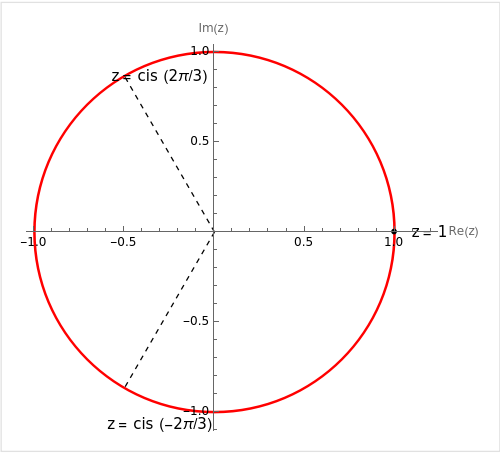
\includegraphics[width = 0.5\textwidth]{rootdemoivre.png}
    \caption{Solutions for $z^3=1$}
\end{figure}
The solutions are shown to lie on the unit circle at intervals of \( \frac{2\pi}{3} \) around the circle.
We find that the number of roots, of course, follows that the number of roots equal to the order of expression.

To generalize, we can see that there are exactly $m$ distinct $mth$ roots of unity, denoted
by
 \begin{equation}
    \boxed{1^{1/m}=e^{i2k\pi/m}=\cos\frac{2k\pi}m+i\sin\frac{2k\pi}m\quad(k=0,1,2, \ldots, m-1).}
 \end{equation}

\begin{theorem}[Solution of \( z^n = a \)] 

    For \( n \in \mathbb{N} \) and \( a \in \mathbb{C} \), the solutions of the equation \( z^n = a \) are called the \textit{n}th roots of \( a \).
\begin{itemize}[leftmargin=*]
    \item The solutions of \( z^n = a \) lie on a circle with center the origin and radius \( |a|^{1/n} \).
    \item There are \( n \) solutions and they are equally spaced around the circle at intervals of \( \frac{2\pi}{n} \). This observation can be used to find all solutions if one is known.
\end{itemize}
\end{theorem}   
More generally, consider any natural number \( n \geq 2 \). Using De Moivre's theorem, we can show that the \( n \)th roots of unity are
\[
1, \, \text{cis}\left(\frac{2\pi}{n}\right), \, \text{cis}\left(\frac{4\pi}{n}\right), \, \ldots, \, \text{cis}\left(\frac{2(n-1)\pi}{n}\right)
\]
So the \( n \)th roots of unity form a geometric sequence with common ratio \( \omega = \text{cis}\left(\frac{2\pi}{n}\right) \).
We can list the terms of this sequence as \( 1, \omega, \omega^2, \ldots, \omega^{n-1} \). The sum of the terms is
\[
1 + \omega + \omega^2 + \ldots + \omega^{n-1} = \frac{\omega^n - 1}{\omega - 1}
\]
since \( \omega^n = 1 \).
\begin{proof}
    The \( n \)th roots of unity are solutions to the equation \( z^n = 1 \). By expressing 1 in polar form as \( 1 \text{cis} 0 \), and applying De Moivre's theorem, \( (r \text{cis} \theta)^n = r^n \text{cis} (n\theta) \), we find that for \( z^n = 1 \), we must have \( z = \text{cis} \left(\frac{2k\pi}{n}\right) \), where \( k \) is an integer from \( 0 \) to \( n-1 \).

These solutions can be written as a sequence where each term after the first is obtained by multiplying the previous term by \( \text{cis} \left(\frac{2\pi}{n}\right) \), making it a geometric sequence with a common ratio of \( \omega = \text{cis} \left(\frac{2\pi}{n}\right) \).

The sum of a geometric sequence with \( n \) terms and a common ratio \( r \neq 1 \) is given by \( S_n = a_1 \frac{1-r^n}{1-r} \). For our sequence, \( a_1 = 1 \) and \( r = \omega \), so the sum is \( S_n = \frac{1-\omega^n}{1-\omega} \). Since \( \omega^n = \text{cis} (2\pi) = 1 \), the numerator becomes \( 1-1 = 0 \), hence the sum \( S_n \) is zero.
\end{proof}

To obtain the \( m \)th roots of an \textit{arbitrary} (nonzero) complex number \( z = re^{i\theta} \), we generalize the idea and, reasoning similarly, conclude that the \( m \) distinct \( m \)th roots of \( z \) are given by
\begin{equation}\label{mthroot}
    \boxed{z^{1/m} = \sqrt[m]{|z|}e^{i(\theta+2k\pi)/m} \quad (k = 0, 1, 2, \ldots, m - 1)}
\end{equation}

Equivalently, we can form these roots by taking any single one such as given in (3) and multiplying by the \( m \)th roots of unity.

\begin{example}
    Find all the cube roots of \( \sqrt{2} + i\sqrt{2} \).
\end{example}
\textbf{Solution:}
The polar form for \( \sqrt{2} + i\sqrt{2} \) is
\[
\sqrt{2} + i\sqrt{2} = 2e^{i\pi/4}.
\]
Putting \( |z| = 2 \), \( \theta = \pi/4 \), and \( m = 3 \) into Eq. \ref{mthroot}, we obtain
\[
(\sqrt{2} + i\sqrt{2})^{1/3} = \sqrt[3]{2}e^{i(\pi/12+2k\pi/3)} \quad (k = 0, 1, 2).
\]
Therefore, the three cube roots of \( \sqrt{2} + i\sqrt{2} \) are \( \sqrt[3]{2}(cos \pi/12 + i \sin \pi/12) \), \( \sqrt[3]{2}(cos 3\pi/4 + i \sin 3\pi/4) \), and \( \sqrt[3]{2}(cos 17\pi/12 + i \sin 17\pi/12) \).
\subsection{Exercises}

\begin{exercise}
    Let \( P(z) = 2z^3 + 9z^2 + 14z + 5 \).

\begin{itemize}
    \item[\textbf{a.}] Use the factor theorem to show that \( z + 2 - i \) is a linear factor of \( P(z) \).
    \item[\textbf{b.}] Write down another complex linear factor of \( P(z) \).
    \item[\textbf{c.}] Hence find all the linear factors of \( P(z) \) over \( \mathbb{C} \).
\end{itemize}
\end{exercise}
\textbf{Solution}

\textbf{a.} By the factor theorem, if \( z + 2 - i \) is a factor of \( P(z) \), then \( P(-2 + i) = 0 \). Calculating this we get:
\begin{align*}
P(-2 + i) &= 2(-2 + i)^3 + 9(-2 + i)^2 + 14(-2 + i) + 5 \\
&= 2(-8 - 12i + 6i^2) + 9(4 - 8i + 2i^2) + 14(-2 + i) + 5 \\
&= 2(-8 - 12i - 6) + 9(4 - 8i - 2) + (-28 + 14i) + 5 \\
&= -28 - 24i - 12 + 36 - 72i - 18 - 28 + 14i + 5 \\
&= 0.
\end{align*}
Thus, \( z + 2 - i \) is a linear factor of \( P(z) \).

\textbf{b.} By the conjugate root theorem, if \( z + 2 - i \) is a root, then its conjugate \( z + 2 + i \) is also a root.

\textbf{c.} Having found two complex roots, we can divide \( P(z) \) by the product of the corresponding factors to find the remaining factor. Let's perform the division (this is a mock example; the actual division should be computed):

% Example of polynomial division (mock)
\begin{align*}
P(z) &= (z + 2 - i)(z + 2 + i)(z - \alpha) \\
\end{align*}

After performing the division, we find that the remaining factor is \( z - \frac{1}{2} \). Thus, the linear factors of \( P(z) \) are:

\[
P(z) = (z + 2 - i)(z + 2 + i)\left(z - \frac{1}{2}\right)
\]

\begin{exercise}
    For a cubic polynomial \(P(x)\) with real coefficients, it is given that \(P(2 + i) = 0\), \(P(1) = 0\) and \(P(0) = 10\). Express \(P(x)\) in the form \(P(x) = ax^3 + bx^2 + cx + d\) and solve the equation \(P(x) = 0\).
\end{exercise}
\textbf{solution:}

Given that \(P(x)\) is a cubic polynomial with real coefficients and \(P(2 + i) = 0\), we know that its conjugate \(P(2 - i) = 0\) as well, due to the complex conjugate root theorem. Moreover, since \(P(1) = 0\), we can write \(P(x)\) as:

\[ P(x) = a(x - (2 + i))(x - (2 - i))(x - 1) \]

Expanding this and simplifying, we get:

\[ P(x) = a((x - 2)^2 + 1)(x - 1) \]

Since \(P(0) = 10\), we can find \(a\) by substituting \(x = 0\):

\[ 10 = a((0 - 2)^2 + 1)(0 - 1) \]
\[ 10 = a(4 + 1)(-1) \]
\[ 10 = -5a \]
\[ a = -2 \]

Thus, the polynomial is:

\[ P(x) = -2((x - 2)^2 + 1)(x - 1) \]
\[ P(x) = -2(x^2 - 4x + 4 + 1)(x - 1) \]
\[ P(x) = -2(x^2 - 4x + 5)(x - 1) \]
\[ P(x) = -2(x^3 - x^2 - 4x^2 + 4x + 5x - 5) \]
\[ P(x) = -2x^3 + 10x^2 - 18x + 10 \]

To solve for \(P(x) = 0\), we now have the equation:

\[ -2x^3 + 10x^2 - 18x + 10 = 0 \]

Since $P(2+i) = 0$, by conjugate root theorem, $p(2-i) = 0$, and we also have $p(1) = 0$.
The order of this expression is 3, by the fundamental algebra theorem, we have found all solutions.

\begin{exercise}
    If \( z = 1 + i \) is a zero of the polynomial \( z^3 + az^2 + bz + 10 - 6i \), find the constants \( a \) and \( b \), given that they are real.
\end{exercise}
\textbf{solution:}

Since \( z = 1 + i \) is a zero, by the Complex Conjugate Root Theorem, \( z = 1 - i \) is also a zero. Substituting \( z = 1 + i \) into the polynomial gives:

\begin{align*}
(1 + i)^3 + a(1 + i)^2 + b(1 + i) + 10 - 6i &= 0 \\
(1 + 3i - 3 - i) + a(1 + 2i - 1) + b + 10 - 6i &= 0 \\
(-2 + 2i) + a(2i) + b + 10 - 6i &= 0 \\
(-2 + (2a - 6)i) + b + 10 &= 0
\end{align*}

For the polynomial to be zero, both the real and imaginary parts must be zero. Therefore, we have two equations:

\begin{align*}
-2 + b + 10 &= 0 \quad \text{(Real part)} \\
2a - 6 &= 0 \quad \text{(Imaginary part)}
\end{align*}

Solving these equations gives us \( a \) and \( b \):

\begin{align*}
b &= -8 \\
a &= 3
\end{align*}

Thus, the constants are \( a = 3 \) and \( b = -8 \).

\begin{exercise}
    Let \( n \) be a positive integer. Prove that \[ \text{arg}(z^n) = n \text{Arg}(z) + 2k\pi, \quad k = 0, \pm1, \pm2, \ldots, \]
    \textbf{for} \( z \neq 0 \)
\end{exercise}
\begin{proof}
    Let's take \( z \in \mathbb{C} \). We can write \( z \) in its polar form as
\[ z = |z|(\cos \theta + i \sin \theta) \]

By definition of arg\( z \) and Arg\( z \) we have: \( \text{arg}(z) = \theta + 2k\pi, k \in \mathbb{Z}, \theta \in [-\pi, \pi] \) and \( \text{Arg}(z) = \text{arg}_{-}(z) = \theta, \theta \in [-\pi, \pi] \).

Now if we take the polar form of \( z^n \), where \( n \in \mathbb{N}, n \neq 0 \), we have
\[ z^n = |z|^n(\cos(n\theta) + i \sin(n\theta)) \]

\[ \Rightarrow \text{arg}(z^n) = n\theta + 2k\pi \]
\[ = n\text{Arg}(z) + 2k\pi, \quad k \in \mathbb{Z} \]

This concludes the proof.
\end{proof}

\begin{exercise}
    Find all the values of the following.
    \begin{enumerate}
        \item[(a)] \( (-16)^{1/4} \)
        \item[(b)] \( 1^{1/5} \)
        \item[(c)] \( i^{1/4} \)
        \item[(d)] \( (1 - \sqrt{3}i)^{1/3} \)
        \item[(e)] \( (i - 1)^{1/2} \)
        \item[(f)] \( \left(\frac{2i}{1+i}\right)^{1/6} \)
    \end{enumerate}
\end{exercise}



\begin{exercise}
    Find all four roots of the equation \( z^4 + 1 = 0 \) and use them to deduce the factorization \( z^4 + 1 = (z^2 - \sqrt{2}z + 1)(z^2 + \sqrt{2}z + 1) \).
\end{exercise}
\textbf{Solution:}

First, we solve the equation:
\begin{align*}
z^4 + 1 &= 0 \\
z^4 &= -1 \\
z &= \sqrt[4]{-1}
\end{align*}

Since \( -1 = \cos \pi + i \sin \pi \), we can find the roots using De Moivre's theorem:
\[ z = \sqrt[4]{\cos \pi + i \sin \pi} = \sqrt[4]{1}(\cos (\pi + 2k\pi)/4 + i \sin (\pi + 2k\pi)/4), \quad k = 0,1,2,3 \]

Thus, the roots are:
\begin{align*}
z_0 &= \cos \frac{\pi}{4} + i \sin \frac{\pi}{4} = \frac{1}{\sqrt{2}} + i \frac{1}{\sqrt{2}} \\
z_1 &= \cos \frac{3\pi}{4} + i \sin \frac{3\pi}{4} = -\frac{1}{\sqrt{2}} + i \frac{1}{\sqrt{2}} \\
z_2 &= \cos \frac{5\pi}{4} + i \sin \frac{5\pi}{4} = -\frac{1}{\sqrt{2}} - i \frac{1}{\sqrt{2}} \\
z_3 &= \cos \frac{7\pi}{4} + i \sin \frac{7\pi}{4} = \frac{1}{\sqrt{2}} - i \frac{1}{\sqrt{2}}
\end{align*}

To show the factorization, we pair the roots:
\begin{align*}
z^4 + 1 &= (z - z_0)(z - z_1)(z - z_2)(z - z_3) \\
&= \left(z - \frac{1}{\sqrt{2}} - i \frac{1}{\sqrt{2}}\right)\left(z + \frac{1}{\sqrt{2}} - i \frac{1}{\sqrt{2}}\right) \\
&\quad \times \left(z + \frac{1}{\sqrt{2}} + i \frac{1}{\sqrt{2}}\right)\left(z - \frac{1}{\sqrt{2}} + i \frac{1}{\sqrt{2}}\right) \\
&= \left(z^2 - \sqrt{2}z + 1\right)\left(z^2 + \sqrt{2}z + 1\right)
\end{align*}

And we have shown the factorization.

\begin{exercise}
    Let \( \alpha \) and \( \beta \) be the mth and nth roots of unity, respectively. We want to show that the product \( \alpha\beta \) is a kth root of unity for some integer \( k \).
\end{exercise}
\textbf{Solution:}

Let's consider \( \alpha \) as the m-th root of unity and \( \beta \) the n-th root of unity. Then we have
\[ \alpha^m = 1 \]
\[ \beta^n = 1 \]

Let's show that \( \alpha\beta \) is a root of unity. If \( \alpha\beta \) is a root of unity then there exists some \( l \in \mathbb{N} \) such that \( (\alpha\beta)^l = 1 \).

For \( l = mn \) (since \( m \) and \( n \) are relatively prime), we have
\[ (\alpha\beta)^l = (\alpha\beta)^{mn} \]
\[ = \alpha^{mn}\beta^{mn} \]
\[ = (\alpha^m)^n(\beta^n)^m \]
\[ = 1^n1^m \]
\[ = 1 \]

Thus, \( \alpha\beta \) is indeed a root of unity, specifically an \( mn \)-th root of unity.

\begin{exercise}
    Let \( m \) and \( n \) be positive integers that have no common factor. Prove that the set of numbers \( (z^{1/n})^m \) is the same as the set of numbers \( (z^m)^{1/n} \). We denote this common set of numbers by \( z^{m/n} \). Show that
\[ z^{m/n} = \sqrt[n]{|z|^m} \left[ \cos \left( \frac{m}{n} (\theta + 2k\pi) \right) + i \sin \left( \frac{m}{n} (\theta + 2k\pi) \right) \right] \]
for \( k = 0, 1, \ldots, n - 1 \).
\end{exercise}
\begin{proof}
    Let's take \( m, n \in \mathbb{N} \) so that they are relatively prime and \( z \in \mathbb{C} \) so that \( \text{Arg}(z) = \theta \). We have:
\begin{align*}
(z^{1/n})^m &= (\sqrt[n]{z})^m = \left( \sqrt[n]{|z|e^{i\theta}} \right)^m \\
&= \left( \sqrt[n]{|z|}e^{i\theta/n} \right)^m \\
&= |z|^{m/n} e^{im\theta/n}
\end{align*}

Now as \( m \) and \( n \) are relatively prime we have
\[ \frac{2k\pi}{n} \frac{m}{n} \quad k = 0, \ldots, n - 1 \]
from where
\begin{align*}
|z|^{m/n} e^{im(\theta + 2k\pi)/n} &= |z|^{m/n} e^{im\theta/n + im2k\pi/n} \\
&= (|z|^m)^{1/n} (e^{im\theta})^{1/n} \\
&= ((|z|^m e^{im\theta})^{1/n} \\
&= (z^m)^{1/n}
\end{align*}

To show the expression we take the previous result and expand it:
\begin{align*}
z^{m/n} &= |z|^{m/n} e^{im\theta/n} \\
&= \sqrt[n]{|z|^m} \left[ \cos \left( \frac{m\theta}{n} + \frac{2km\pi}{n} \right) + i \sin \left( \frac{m\theta}{n} + \frac{2km\pi}{n} \right) \right] \\
&= \sqrt[n]{|z|^m} \left[ \cos \left( \frac{m}{n} (\theta + 2k\pi) \right) + i \sin \left( \frac{m}{n} (\theta + 2k\pi) \right) \right]
\end{align*}
\end{proof}


\begin{exercise}
    Use the conclusion in last problem to evaluate $(i-i)^\frac{3}{2}$.
\end{exercise}
\textbf{Solution:}
It has been shown that
\begin{equation}
    \boxed{ z^{m/n} = \sqrt[n]{|z|^m}\left[\cos\left(\frac{m}{n}(\theta + 2k\pi)\right) + i\sin\left(\frac{m}{n}(\theta + 2k\pi)\right)\right]}
\end{equation}
We have:
\[ z = (1 - i)^{3/2} \Rightarrow m = 3, n = 2 \]
\[ |z| = \sqrt{1^2 + (-1)^2} = \sqrt{2} \]
\[ \theta = \text{Arg} z = 2\pi - \cot^{-1}\left(\frac{-1}{1}\right) = \frac{7\pi}{4} \]

When we put everything in the formula we get
\[ z = \sqrt[2]{\sqrt{2}^3}\left[\cos\left(\frac{3}{2}\left(\frac{7\pi}{4} + 2k\pi\right)\right) + i\sin\left(\frac{3}{2}\left(\frac{7\pi}{4} + 2k\pi\right)\right)\right], k = 0, 1 \]
\[ z = \sqrt[2]{2^{3/2}}\left[\cos\left(\frac{21\pi}{8} + \frac{3k\pi}{2}\right) + i\sin\left(\frac{21\pi}{8} + \frac{3k\pi}{2}\right)\right], k = 0, 1 \]
\[ z_0 = 2^{3/4}\left[\cos\left(\frac{21\pi}{8}\right) + i\sin\left(\frac{21\pi}{8}\right)\right] \]
\[ z_1 = 2^{3/4}\left[\cos\left(\frac{21\pi}{8} + \frac{3\pi}{2}\right) + i\sin\left(\frac{21\pi}{8} + \frac{3\pi}{2}\right)\right] \]
%------------------------------------------------


